\chapter{Conceptos B\'asicos}
%\minitoc
  Un n\'umero considerable de problemas de la vida real requieren de la optimizaci\'on de dos o m\'as objetivos a la vez, 
  los cuales, en general, est\'an en conflicto unos con otros al mismo tiempo. En este cap\'itulo se describen algunos 
  conceptos b\'asicos de algoritmos evolutivos, de la optimizaci\'on multi-objetivo y del algoritmo de c\'umulos de 
  part\'iculas que servir\'an como marco te\'orico para el resto de la tesis. En este cap\'itulo se proporcionan tambi\'en 
  las principales caracter\'isticas del indicador llamado hipervolumen, as\'i como un breve estado 
  del arte sobre los algoritmos evolutivos multi-objetivo m\'as relacionados con este trabajo de tesis.

  \section{Conceptos de computaci\'on evolutiva}
  
  La computaci\'on evolutiva consiste en t\'ecnicas estoc\'asticas de b\'usqueda y optimizaci\'on inspiradas en el 
  \textit{neodarwinismo}. A estas t\'ecnicas se les conoce gen\'ericamente como \textit{Algoritmos} \textit{Evolutivos} 
  y han tenido mucho  \'exito en la soluci\'on de problemas de optimizaci\'on, debido a que presentan las siguientes 
  caracter\'isticas \cite{vicente06}:
  
  \begin{itemize}
  \item No requieren de conocimientos espec\'ificos sobre el problema.
  \item Pueden actuar como eficaces optimizadores globales, ya que son menos propensos a quedar atrapados en 
  \'optimos locales.
  \item Son f\'aciles de comprender e implementar en forma secuencial y paralela.
  \item Se pueden hibridizar con otras t\'ecnicas de optimizaci\'on (por ejemplo, t\'ecnicas de programaci\'on 
  matem\'atica).
  \end{itemize}

  El \textit{neodarwinismo} se compone de tres aspectos b\'asicos:
  
  \begin{itemize}
   \item \textbf{La teor\'ia de la evoluci\'on de \textit{Darwin}}. La contribuci\'on de Darwin a los conocimientos 
   cient\'ificos acerca de la evoluci\'on se centr\'o directamente en la identificaci\'on del mecanismo principal de la 
   evoluci\'on, llamado \textit{selecci\'on} \textit{natural}. Esta teor\'ia establece que las condiciones del medio 
   favorecen o dificultan la reproduci\'on de los individuos para adaptarse al medio y sus cambios constantes. Esta 
   adaptabilidad que presentan los individuos hacia los cambios del medio se sostiene con la afirmaci\'on 
   de que los descendientes tienen variaciones no aleatorias y no deterministas que son, en parte, heredables y otras
   variaciones que dan lugar a una mejor sobrevivencia y \'exito reproductivo, haciendo que a lo largo de las generaciones 
   se produzca el fen\'omeno evolutivo \cite{darwin59}.
 
   \item \textbf{La teor\'ia de Germoplasma de \textit{Weismann}}. \cite{Weismann93} propuso la teor\'ia de germoplasma 
   como un mecanismo de herencia en la teor\'ia de Darwin. Esta teor\'ia distingue dos componentes en los individuos: 
   el primero, son las c\'elulas germinales que contienen informaci\'on hereditaria que no puede ser alterada por las 
   habilidades adquiridas durante la vida del individuo, es decir, son las c\'elulas que dan origen a la descendencia; 
   el segundo, son las c\'elulas som\'aticas las responsables de las funciones corporales.
   
   \item \textbf{La Gen\'etica Mendeliana o Leyes de Mendel}. Las leyes de Mendel son un conjunto de reglas sobres la 
   transmisi\'on por herencia entre los individuos (padres a hijos). Estas leyes fueron derivadas por \cite{Mendel01}:
   
   \begin{enumerate}
    \item \textbf{Ley de la segregaci\'on}: establece que durante la formaci\'on de los gametos cada alelo de un par se 
    separa del otro miembro para determinar la constituci\'on gen\'etica del gameto.
    \item \textbf{Ley de la segregaci\'on independiente}: durante la formaci\'on de los gametos la segregaci\'on de los 
    alelos de un par es independiente de la segregaci\'on de los alelos de otro par.
    \item \textbf{Ley de la dominancia}: cuando un individuo tiene dos alelos diferentes para un rasgo (un alelo es 
    dominante y otro recesivo), el alelo dominante se expresa mientras que el alelo recesivo se mantiene oculto.
   \end{enumerate}

   De acuerdo con el \textit{neodarwinismo}, se tienen cuatro procesos estoc\'asticos que actu\'an en todas las especies
   \cite{hoffman89}:
   \begin{itemize}
    \item \textbf{La reproducc\'on}: es la formaci\'on de nuevos individuos a partir de otros preexistentes y, por tanto, 
    pueden aparecer individuos diferentes a los de los progenitores, es decir, es un proceso que permite la creaci\'on 
    de nuevos individuos.
    \item \textbf{La mutaci\'on}: son cambios al azar que se producen en la composici\'on gen\'etica de un individuo. Se 
    originan en los cromosomas, por lo que se pueden transmitir a la descendencia durante la reproducci\'on. Consisten 
    generalmente en que un gen sufre alguna modificaci\'on. 
    \item \textbf{La competencia}: es la interacci\'on entre los individuos que pertenecen a una comunidad, debido a la 
    disponibilidad de ciertos recursos limitados.
    \item \textbf{La selecci\'on}: las combinaciones peor adaptadas al medio se eliminan, mientras que las mejor adaptadas 
    ser\'an m\'as abundantes, porque sus portadores se reproducir\'an m\'as eficientemente, las transmitir\'an a su descendencia 
    y aumentar\'an su proporci\'on en la poblaci\'on. 
   \end{itemize}
  \end{itemize}
  
  A continuaci\'on se definen algunos conceptos b\'asicos de la computaci\'on evolutiva.
  
  \subsection{Representaci\'on}
  
  Se denomina \textit{cromosoma} a una estructura de datos que contiene una cadena de variables de decisi\'on de alg\'un 
  problema (figura \ref{fig:cromosoma}). Usualmente es una cadena binaria, pero tambi\'en es posible usar una cadena con 
  valores enteros o reales.

  \begin{figure}[H]
	\centering
	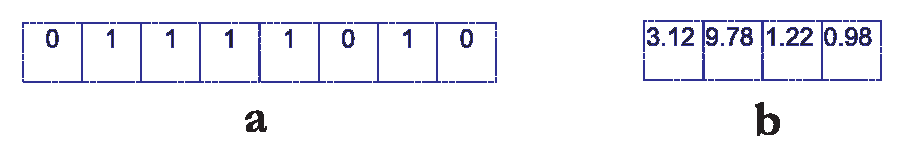
\includegraphics[scale=0.45]{Cap2/1-16.eps}
	  \caption{Ejemplo de un cromosoma binario (a) y otro real (b).}
      \label{fig:cromosoma}
      \end{figure}
  
  Llamamos \textit{gene} a una subcadena del cromosoma que codifica, com\'unmente, a un solo par\'ametro de dise\~no. Estos genes toman 
  ciertos valores, llamados \textit{alelos}, de alg\'un alfabeto gen\'etico. De esta manera, si usamos una representacion binaria, 
  los alelos 
  pueden tomar el valor de $0$ o de $1$. Un \textit{locus} define la posici\'on de un gene dentro del cromosoma (figura \ref{fig:gene}).

  \begin{figure}[H]
	\centering
	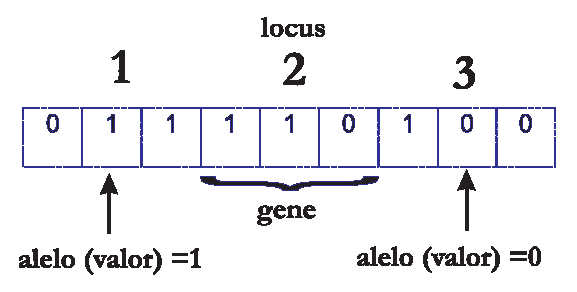
\includegraphics[scale=0.70]{Cap2/1-17.eps}
	  \caption{Cromosoma binario constituido por tres genes.}
      \label{fig:gene}
      \end{figure}
  
  Se denomina \textit{genotipo} a la codificaci\'on (por ejemplo, binaria, entera o real) de los par\'ametros de decisi\'on. Mientras 
  que \textit{fenotipo} es la decodificaci\'on del genotipo, con el fin de obtener los valores de los par\'ametros usados como entrada 
  en la funci\'on objetivo del problema que se trata (figura \ref{fig:genotipo}).

  \begin{figure}[H]
	\centering
	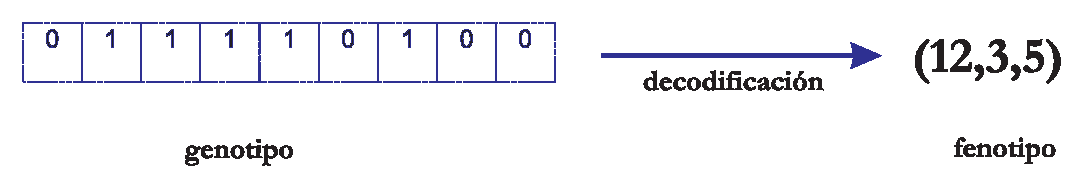
\includegraphics[scale=0.70]{Cap2/1-18.eps}
	  \caption{Decodificaci\'on del genotipo al fenotipo.}
      \label{fig:genotipo}
      \end{figure}
  
  Un \textit{individuo} es una soluci\'on potencial al problema que se trata. Cada individuo contiene un cromosoma. A un conjunto de individuos 
  se le nombra \textit{poblaci\'on}. La \textit{aptitud} de un individuo es la evaluaci\'on de la funci\'on de aptitud e indica qu\'e
  tan bueno es el individuo (es decir, la soluci\'on al problema) con respecto a los dem\'as.

  \subsection{Operadores evolutivos}
  
  Existe una amplia variedad de operadores que se han empleado en los algoritmos evolutivos. Algunos de ellos est\'an 
  dise\~nados especialmente para una clase particular de problemas. A continuaci\'on se describen los m\'as usados com\'unmente:
  
  \begin{itemize}
   \item \textbf{Selecci\'on}: la selecci\'on determina la probabilidad de elegir un individuo para que produzca descendencia por medio 
   de la recombinaci\'on y la mutaci\'on. El esquema de selecci\'on es una de las partes cruciales de un algoritmo evolutivo, puesto 
   que sesga la b\'usqueda de manera que eventualmente se llegue a la soluci\'on \'optima (o su proximidad).
   \item \textbf{Recombinaci\'on}: el operador de recombinaci\'on (cruza) tiene la finalidad de heredar la informaci\'on (genes) 
   de dos o m\'as padres a la descendencia. En la computaci\'on evolutiva la cruza entre cromosomas se simula intercambiando segmentos 
   de cadenas lineales de longitud fija. Lo usual es que las t\'ecnicas de cruza se apliquen sobre representaciones binarias; sin embargo, 
   con las modificaciones adecuadas, se pueden generalizar a alfabetos de cardinalidad mayor.
   \item \textbf{Mutaci\'on}: la mutaci\'on consiste en peque\~nas modificaciones al cromosoma de un individuo. En los 
   algoritmos gen\'eticos la mutaci\'on es considerada un operador secundario.
  \end{itemize}
  
  \subsection{Principales paradigmas}
  
  Actualmente existen, principalmente, tres paradigmas inspirados en los principios del \textit{neodarwinismo}: los \textit{algoritmos}
  \textit{gen\'eticos}, la \textit{programaci\'on} \textit{evolutiva} y las \textit{estrategias} \textit{evolutivas}. De manera gen\'erica, 
  a los algoritmos de la computaci\'on evolutiva se les llama \textit{algoritmos evolutivos}. Estas tres t\'ecnicas tienen en com\'un la 
  reproducci\'on, la variaci\'on aleatoria, la competencia y la selecci\'on de individuos contendientes dentro de una poblaci\'on. 
  
\begin{itemize}
 \item \textbf{Estrategias Evolutivas}: este modelo enfatiza los nexos conductuales entre padres e hijos, en lugar del nexo gen\'etico. 
 \'Estas fueron concebidas para construir sistemas capaces de resolver problemas de optimizaci\'on complejos en los que las variables
 son n\'umeros reales. Por ello, la representaci\'on natural fue un vector de genes con valores reales, el cual era manipulado, principalmente, 
 por operadores de mutaci\'on que perturbaban dichos valores reales \cite{Back97}.
 
 La primera versi\'on de una estrategia evolutiva, nombrada $(1+1)$-EE, crea un solo hijo a partir de un solo padre, y ambos compet\'ian
 para sobrevivir; el peor individuo era eliminado, mientras que el mejor se manten\'ia para la siguiente generaci\'on. En la $(1+1)$-EE, 
 a partir de un padre $x^{t}=(x_1, \ldots, x_n )$, el hijo se genera mediante la expresi\'on:

 \[x^{t+1}_i=x^{t} + N_i(0, \sigma^{t}_i)\]
 
donde $t$ se refiere a la generaci\'on actual, $i = 1, \ldots, n$ es la $i$-\'esima componente de los vectores $x$, $N$, $\sigma$ y
$\sigma^{t}_i$ es un n\'umero aleatorio gaussiano con media cero y desviaci\'on est\'andar $\sigma_i$ . Los n\'umeros aleatorios 
son generados de manera independiente.
 
 \item \textbf{Programaci\'on Evolutiva}: propuesta por Lawrence Fogel consideraba que el comportamiento inteligente requiere de dos 
 habilidades: la primera, a trav\'es de un organismo para poder hacer predicciones correctas dentro de su ambiente; y la segunda, 
 es la capacidad de traducir estas predicciones en una respuesta adecuada para una 
 meta dada. Los aut\'omatas de estados finitos fueron la representaci\'on ideal para modelar este comportamiento \cite{Fogel64}. 
 
 \item \textbf{Algoritmos Gen\'eticos}. Propuestos por \cite{Holland75}. Hay tres caracter\'isticas principales que los distinguen 
 de los dem\'as algoritmos evolutivos: la representaci\'on de los individuos (cadena binaria); el m\'etodo de selecci\'on (selecci\'on 
 proporcional); y el uso de la cruza como el operador principal para modificar al individuo. En este caso, la mutaci\'on es un operador 
  secundario.

\end{itemize}

\section{Optimizaci\'on multi-objetivo}
  
      Se define el problema de optimizaci\'on multi-objetivo como: ``La tarea de encontrar un vector de variables 
      de decisi\'on que satisfaga restricciones y optimice un vector de funciones objetivo. Esas funciones, generalmente est\'an
      en conflicto unas con otras y, describen matem\'aticamente un criterio de desempe\~no. Por lo tanto, el t\'ermino 
      optimizar significa encontrar un vector soluci\'on con valores aceptables para todas las funciones objetivo'' \cite{EASMC85}. 
      Los problemas multi-objetivo son aquellos en los que se deben optimizar $k \geq 2$ funciones objetivo simult\'aneamente. 
      El proceso de optimizaci\'on puede significar la maximizaci\'on de las $k$ funciones, la minimizaci\'on de las $k$ 
      funciones o una combinaci\'on de maximizaci\'on y minimizaci\'on de estas funciones.

      \begin{definicion}[Problema de Optimizaci\'on]
	  Un problema de optimizaci\'on multi-objetivo se define como la tarea de minimizar (o maximizar) 
	  
	  \[F\left(\vec{x}\right)=\left(f_1\left(\vec{x}\right), \ldots,f_k\left(\vec{x}\right) \right),\]
	  
	  {\setlength{\parindent}{0pt}
	  
	  donde $k\geq 2$ es el n\'umero de funciones a optimizar, sujetas a $g_i\left(\vec{x}\right) \leq 0 $ (restricciones de 
	  desigualdad) y $h_j\left(\vec{x}\right) = 0 $ (restricciones de igualdad) con $i = \left\{1, \ldots, m \right\}$, $j = \left\{1, \ldots, n \right\}$ 
	  y $\vec{x} \in \Psi $, donde $\vec{x}$ es un vector $n$-dimensional de variables de decisi\'on ($\vec{x} = \left(x_1 , \ldots, x_n \right) \in \Psi$). 
	  Las restricciones $g_i\left(\vec{x}\right) \leq 0$ y $h_j\left(\vec{x}\right) = 0$ deben ser satisfechas 
	  al mismo tiempo que se minimiza (o maximiza) $F\left(\vec{x}\right)$ y $\Psi $ contiene todos los posibles 
	  $\vec{x}$ que pueden ser usados para satisfacer la evaluaci\'on de $F\left(\vec{x}\right)$.
	  }
      \end{definicion}

      El vector de variables de decisi\'on puede ser continuo o discreto mientras que las $k$ funciones pueden ser 
      lineales o no, as\'i como continuas o discretas. La funci\'on de evaluaci\'on $F:\Psi \rightarrow \Omega$ es una transformaci\'on 
      del vector de variables de decisi\'on $\vec{x} = \left(x_1 , \ldots, x_n \right)$ en un vector de respuesta 
      $\vec{y} = \left(y_1 , \ldots, y_k \right)$. La figura ~\ref{fig:multiobj} muestra un problema de dos objetivos con dos variables.
      
      \begin{figure}
	\centering
	\includegraphics[scale=0.6]{Cap2/1-1.eps}
	  \caption{Un problema de dos objetivos con dos variables}
      \label{fig:multiobj}
      \end{figure}
            
      Cuando el problema es multi-objetivo existe un conflicto que ocasiona que la mejora en alg\'un objetivo provoque 
      el deterioro de otros. Por lo tanto, un problema de optimizaci\'on multi-objetivo consiste en encontrar el mejor 
      compromiso (balance) entre todos los objetivos. Las soluciones que representan los mejores compromisos entre los 
      objetivos se denominan \'optimos de Pareto.  
      
      \begin{definicion}[Optimalidad de Pareto]
	  Una soluci\'on $\vec{x}^*\in \Psi$ es un \'optimo de Pareto con respecto a $\Psi$ si y s\'olo si no existe 
	  $\vec{x}\in \Psi$, para la cual $\vec{v} = F\left(\vec{x}\right)=\left(f_1\left(\vec{x}\right), \ldots,f_k\left(\vec{x}\right) \right)$ 
	  domina a $\vec{u}^*=F\left(\vec{x}^*\right)=\left(f_1\left(\vec{x}^*\right), \ldots,f_k\left(\vec{x}^*\right) \right)$.
      \end{definicion}
      
      \begin{definicion}[Dominancia de Pareto]
	  Un vector $\vec{u} = \left(u_1, \ldots, u_k \right)$ se dice que domina a $\vec{v} = \left(v_1, \ldots, v_k \right)$,
	  denotado por $\vec{u} \preceq \vec{v}$, si y s\'olo si $\vec{u}$ es parcialmente menor que $\vec{v}$, es decir, 
	  $\forall i \in \left\{1, \ldots, k \right\}: u_i \leq v_i \wedge \exists i \in \left\{1, \ldots, k\right\}: u_i < v_i$.
      \end{definicion}
    
      La figura \ref{fig:paretodominance} muestra gr\'aficamente la dominancia de Pareto para un problema de optimizaci\'on
      con dos objetivos en el cual $A \preceq C$ tal que $A$ es mejor en ambas funciones, $A \preceq E$ tal que $A$ es igual con respecto 
      a $f_2$ pero es mejor con respecto a $f_1$, $B \preceq E$ tal que $B$  es igual con respecto a $f_1$ pero mejor con respecto a 
      $f_2$, $B\preceq D$ tal que B es mejor en ambas funciones, y $A$ y $B$ son incomparables ($A$ y $B$ son \'optimos de Pareto).
       
       \begin{figure}
	\centering
	\includegraphics[scale=0.6]{Cap2/1-4.eps}
	  \caption{Dominancia de Pareto}
      \label{fig:paretodominance}
      \end{figure}
       
      \begin{definicion}[Conjunto de \'optimos de Pareto]
	Para un problema multi-objetivo determinado $F\left(\vec{x}\right)$, el conjunto de \'optimos de Pareto, denotado por $P^*$ 
	o $P_{real}$, est\'a definido como:	
	\[
	P^*= \left\{ \vec{x} \in \Psi |\hspace{0.3cm} \nexists \vec{y}\in \Psi \hspace{0.7cm} F\left(\vec{y}\right)\preceq F\left(\vec{x}\right) \right\}\]
      \end{definicion}
      
      Los elementos del conjunto de \'optimos de Pareto tienen vectores objetivo que no pueden ser mejorados sin empeorar al menos otro
      objetivo. Los vectores objetivo de las soluciones \'optimas de Pareto se denominan vectores (o soluciones) \textit{no dominados}.
      Los vectores de las funciones objetivo correspondientes al conjunto de \'optimos de Pareto conforman el denominado frente de Pareto 
      ($\mathcal{F}^*$).
      
      \begin{definicion}[Frente de Pareto]
      Para un problema multi-objetivo determinado $F\left(\vec{x} \right)$, siendo su conjunto de \'optimos de Pareto ($P^*$) , el Frente 
      de Pareto $\mathcal{F}^*$ o $\mathcal{F}_{real}$, est\'a definido como (ver figura \ref{fig:pareto}):
      
	  \[\mathcal{F}^*=\left\{ \vec{u} = F\left(\vec{x}\right) | \hspace{0.3cm} \vec{x}\in P^*\right\}\]
      \end{definicion}
      
      \begin{figure}
	\centering
	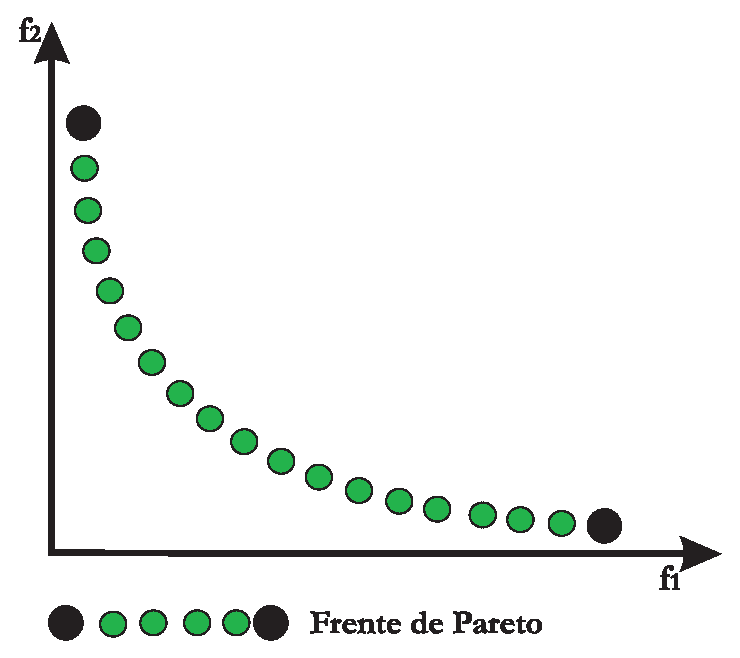
\includegraphics[scale=0.65]{Cap2/1-2.eps}
	  \caption{Frente de Pareto}
      \label{fig:pareto}
      \end{figure}
      
      \begin{definicion}[Vector Ideal y vector de Nadir]
      Para un problema multi-objetivo determinado $F\left(\vec{x}\right)$, siendo su conjunto de \'optimos de Pareto, $P^*$, 
      el vector ideal se define como (ver figura \ref{fig:ideanadir}):
      
      \[  f_{ideal}= \left(^{\min}_{\vec{x}\in P^*}f_1\left(\vec{x}\right), \ldots, ^{\min}_{\vec{x}\in P^*}f_k\left(\vec{x}\right) \right)\]
      
      Si el vector ideal de un problema es alcanzabe, entonces los objetivos del problema no est\'an en conflicto 
      y la soluci\'on del problema es \'unica. Por lo tanto, cada objetivo del problema puede ser optimizado por separado,
      sin requerirse el uso de un algoritmo evolutivo multi-objetivo.
      De manera similar, el vector de Nadir se define como (ver figura \ref{fig:ideanadir}):
      
      \[  f_{nadir}= \left(^{\max}_{\vec{x}\in P^*}f_1\left(\vec{x}\right), \ldots, ^{\max}_{\vec{x}\in P^*}f_k\left(\vec{x}\right) \right)\]
      
      Este vector contiene, entonces, los peores valores de las funciones objetivo y suele usarse (junto al vector ideal)
      para acotar el frente de Pareto.      
      
      \end{definicion}
      
      \begin{figure}
	\centering
	\includegraphics[scale=0.65]{Cap2/1-3.eps}
	  \caption{Vector Ideal y vector de Nadir}
      \label{fig:ideanadir}
      \end{figure}
      
      \subsection{M\'etricas para evaluar la eficacia}
      \label{sec:metric}
      Al trabajar en optimizaci\'on multi-objetivo, se tienen que tomar en cuenta dos nociones importantes: la convergencia y la 
      dispersi\'on. Para medir la convergencia, se debe de estimar qu\'e tan lejos est\'an las soluciones que generamos del
      verdadero frente de Pareto y para medir la dispersi\'on, se debe estimar qu\'e tan uniformemente est\'an distribuidos 
      las soluciones a lo largo del frente de Pareto. Para medir la convergencia se pueden usar medidas como las siguientes:
      
      \begin{definicion} [Distancia Generacional Invertida (IGD)]
      Determina cu\'an lejos, en promedio, se encuentra el verdadero frente de Pareto, del frente obtenido por el algoritmo.
      Esta m\'etrica evita algunos problemas que posee la denominada Distancia Generacional, en particular, en los casos en 
      los que el frente obtenido posee pocos puntos, pero agrupados en una sola regi\'on \cite{Veldhuizen98}. 
      Su definici\'on es la siguiente:

      \[
	IGD = \frac{1}{N} \cdot \sqrt{\sum^{N}_{i=1}{d^2_i}},
      \]
      {\setlength{\parindent}{0pt}
      donde $N$ es la cantidad de puntos del verdadero frente de Pareto, $d_i$ la distancia euclidiana (medida en el espacio 
      de las funciones objetivo) entre cada punto del verdadero frente, al punto m\'as cercano del frente obtenido. Un valor 
      $IGD = 0$ indica que el frente obtenido es el verdadero frente de Pareto, cualquier otro valor indica que el frente obtenido 
      se desv\'ia del verdadero frente de Pareto.
      }
      \end{definicion}
  
      \begin{definicion}[Cobertura de Conjuntos ($\mathcal{C}$)]
	  Determina la cobertura relativa de un conjunto, con respecto a otro. Fue propuesta por \cite{Zitzler2000} para 
	  valorar cuantitativamente cu\'anto un conjunto cubre o domina a otro. Si $A$ y $B$ son dos conjuntos no dominados,
	  la m\'etrica de cobertura de $\mathcal{C}(A,B)$ calcula la fracci\'on de vectores en $B$ que son dominados 
	  d\'ebilmente por los vectores de $A$. Se define como:

	  \[
	      \mathcal{C}\left(A, B \right) = \frac{|\vec{b} \in B; \exists \vec{a} \in A: \vec{a}\preceq \vec{b}|}{|B|}
	  \]
	  
	  Si todos los vectores en $B$ son dominados o son iguales a los vectores en $A$, entonces $\mathcal{C}$ es igual a uno. 
	  Si ninguno de los vectores en $B$ es dominado o igual a alg\'un vector de $A$, entonces $\mathcal{C}$ es igual a cero. 
	  Lo ideal es que $\mathcal{C} \left(A, B\right)$  y $\mathcal{C} \left(B, A \right)$ se consideren de manera separada, 
	  ya que $\mathcal{C}\left(A, B\right)$ no es equivalente a $1- \mathcal{C}\left(B, A\right)$
      \end{definicion}
      
      \begin{definicion}[Dispersi\'on o Espaciamiento (Spread) (S)]
	 Determina la dispersi\'on de los puntos sobre el frente. Fue utilizada por \cite{deb02} para conocer 
	 c\'omo est\'an distribuidas las soluciones a lo largo del frente de Pareto. Se define como:
	 
	 \[S= \frac{d_f + d_l + \sum^{N-1}_{i=1}{|d_i-d^{'}|}}{d_f + d_l + \left(N -1\right)\cdot d^{'}}\]
  
      donde $N$ es la cantidad de puntos del frente, $d_i$ es la distancia euclidiana entre soluciones consecutivas, 
      $d^{'}$ es el valor medio de todas las distancias y, $d_f$ y $d_l$ son las distancias euclidianas a los extremos 
      del frente de Pareto. Un valor $S = 0$ indica la distribuci\'on ideal (dispersi\'on perfecta).
      \end{definicion}   
      
      La dispersi\'on indica qu\'e tan bien est\'an distribuidas las soluciones en el verdadero frente de Pareto (o su aproximaci\'on).
      Este indicador es importante, ya que ofrece m\'as opciones para la toma de decisiones al momento de elegir una o m\'as soluciones 
      no dominadas.
  
  \subsection{Algoritmos evolutivos multi-objetivo}

  Hoy en d\'ia existen diversas t\'ecnicas de programaci\'on matem\'atica para resolver problemas de optimizaci\'on multi-objetivo 
  \cite{Miettinen98, EASMC85}. Sin embargo, la complejidad de muchos problemas de optimizaci\'on multi-objetivo del mundo real vuelven 
  a estas t\'ecnicas inadecuadas o incluso inaplicables para resolverlos. La complejidad de estos problemas se debe, por ejemplo a: 
  la multimodalidad, la alta dimensionalidad del espacio de b\'usqueda, a la discontinuidad de las funciones objetivo, a desconexiones 
  tanto en el espacio de la variables de decisi\'on como en el de las funciones objetivo, entre otras causas.

  Rosenberg plante\'o utilizar un m\'etodo gen\'etico de b\'usqueda para resolver problemas de optimizaci\'on
  multi-objetivo por primera vez, pero no lleg\'o a desarrollar un algoritmo, dado que transform\'o el problema 
  bi-objetivo de su inter\'es en uno mono-objetivo \cite{Rosenberg67}. La primera implementaci\'on de lo que 
  actualmente se conoce como un algoritmo evolutivo multi-objetivo fue propueta por \cite{Schaffer84}. 

  Los algoritmos evolutivos resultan particularmente adecuados para resolver problemas de optimizaci\'on multi-objetivo gracias a que
  trabajan simult\'aneamente con un conjunto de soluciones potenciales (es decir, la poblaci\'on). Esta caracter\'istica les permite 
  encontrar varias soluciones del conjunto de \'optimos de Pareto en una sola ejecuci\'on. Tambi\'en, son menos sensibles a la forma o 
  continuidad del frente de Pareto. Adicionalmente, son f\'aciles de usar y no requieren informaci\'on espec\'ifica del problema a resolverse.

  Los algoritmos evolutivos y los algoritmos evolutivos multi-objetivo son estructuralmente similares. La diferencia principal es que 
  los segundos utilizan un esquema de selecci\'on que debe considerar $k$ ($k \geq 2$) funciones objetivo, adem\'as de contar
  con un estimador densidad en el espacio de las funciones objetivo que sesga el mecasnimo de selecci\'on de manera 
  que se mantenga diversidad en la poblaci\'on. 
  Sin embargo, el operador de selecci\'on espera un solo valor de aptitud. La forma m\'as sencilla de mantener 
  la estructura de un algotirmo evolutivo simple al abordar problemas multi-objetivo (si bien, no es la m\'as adecuada) consiste en 
  transformar el vector de aptitudes en un valor escalar. En el algoritmo \ref{alg:AEb} se describe una estructura b\'asica de un 
  algoritmo evolutivo multi-objetivo, de este tipo. N\'otese que este algoritmo no incluye un estimador de densidad.
  
  \begin{algorithm}
      \begin{algorithmic}[1]			
	\STATE $t \leftarrow 0$.
	\STATE Generar aleatoriamente la poblaci\'on inicial $P^t$.
	\WHILE{$t < max_{Gen}$}
	\STATE Para cada individuo $\vec{x} \in P^t$ calcular el valor escalar de aptitud $F(\vec{x})$.
	\STATE Seleccionar de $P^t$ un grupo de padres $P'^t$ bas\'andose en la aptitud.
	\STATE Recombinar los individuos de $P'^t$ para obtener $P''^t.$
	\STATE Mutar los individuos de $P''(t)$ para obtener $P'''^t$.
	\STATE $P^{t+1 } \leftarrow P'''^t$.
	\STATE $t\leftarrow t +1$.
	\ENDWHILE 
  \end{algorithmic}
  \caption{Estructura b\'asica de un algoritmo evolutivo multi-objetivo agregativo}
  \label{alg:AEb}
  \end{algorithm}

  En general, existen diferentes esquemas para manejar varias funciones objetivo en la selecci\'on: los basados en agregaci\'on, los basados 
  en poblaciones, y los basados en el concepto de dominancia de Pareto \cite{Zitzler99}. Otro componente fundamental de los algoritmos
  evolutivos multi-objetivo modernos es el elitismo.

  Actualmente hay dos formas principales de llevar a cabo la implementaci\'on del elitismo en un algoritmo evolutivo multi-objetivo. La primera,
  es combinar la poblaci\'on anterior y la descendencia o la poblaci\'on nueva, y posteriormente aplicar una selecci\'on determinista 
  en lugar de reemplazar la vieja poblaci\'on por la descendencia \cite{deb02}. La segunda, es mantener una poblaci\'on secundaria 
  llamada archivo hist\'orico (poblaci\'on secundaria, poblaci\'on elitista o archivo externo) en el cual se retienen las soluciones no 
  dominadas encontradas en el transcurso del proceso de b\'usqueda \cite{Zitzler99}(ver figura \ref{fig:elitismo}). En muchos problemas 
  de optimizaci\'on multi-objetivo, el conjunto de \'optimos de Pareto es muy grande. Por ello, se debe aplicar una estrategia para decidir 
  la entrada de la nuevas soluciones al archivo y evitar que el archivo crezca indefinidamente.
  
    \begin{figure}[H]
	\centering
	\includegraphics[scale=0.60]{Cap2/1-19.eps}
	  \caption{Dos esquemas para llevar a cabo el elitismo.}
      \label{fig:elitismo}
      \end{figure}
  
  \subsection{Clasificaci\'on}
  
  Existen diferentes maneras de clasificar a los algoritmos evolutivos multi-objetivo. Quiz\'as la taxonom\'ia m\'as simple, 
  es la basada en el tipo de mecanismo de selecci\'on que usan \cite{EASMC}:
  
  \begin{itemize}
   \item \textbf{Enfoques basados en agregaci\'on}. Esta t\'ecnica simplemente combina todos los objetivos 
   en un valor escalar, es decir, transforman 
   un problema de optimizaci\'on multi-objetivo en un problema de optimizaci\'on mono-objetivo. Para ello se usa la siguiente 
   expresi\'on: 
   
	\[ \min {\sum^{k}_{i=1}{w_i\cdot f_i\left(\vec{x}\right)}}\]
   
   donde $w_i > 0$ son los coeficientes de ponderaci\'on que representan la importacia de cada cada objetivo $k$ del
   problema. Usualmente se presupone que:
   
   \[\sum^{k}_{i=1}{w_i}=1\]
   
   Las funciones agregativas lineales tienen diversos inconvenientes, entre los que destaca el hecho de no 
   poder generar partes no convexas del frente de Pareto. Las funciones agregativas no lineales no tienen esta limitante,
   pero no son muy comunes en la literatura especializada. Pese a sus limitantes, las funciones agregativas han sido utilizadas
   con \'exito en problemas combinatorios multi-objetivo.
   
   \item \textbf{Enfoques basados en poblaci\'on}. En este tipo de enfoque, la poblaci\'on se utiliza para la diversificaci\'on de la b\'usqueda, 
   pero el concepto de dominancia de Pareto no se incorporan directamente en el proceso de selecci\'on. Un ejemplo cl\'asico es el 
   algoritmo \textbf{VEGA} (\textit{Vector Evaluated Genetic Algorithm}) \cite{Schaffer84}. VEGA consiste en un algoritmo gen\'etico 
   con un mecanismo de selecci\'on modificado. En cada generaci\'on, se crea un n\'umero de sub-poblaciones de acuerdo con una 
   selecci\'on proporcional a cada objetivo por cada funci\'on a la vez. Estas sub-poblaciones son luego mezcladas entre s\'i para 
   obtener una nueva poblaci\'on, en la que el algoritmo gen\'etico aplica los operadores de cruza y mutaci\'on. VEGA tiene varios 
   problemas, del cual se puede destacar el que su esquema de selecci\'on se opone al concepto de dominancia de Pareto.
   
   \item \textbf{Enfoques basados en optimilidad de Pareto}. En este tipo de enfoque, se consideran los algoritmos evolutivos multi-objetivo que 
   incorporan el concepto de Pareto en su mecanismo de selecci\'on. Los siguentes algoritmos evolutivos son un conjunto representativo 
   que utilizan este enfoque en los \'ultimos a\~nos:
   
   \begin{itemize}
    \item \textbf{PAES (\textit{The Pareto Archived Evolution Strategy})}: este m\'etodo consiste en una estrategia evolutiva (1+1),
    en combinaci\'on con un archivo hist\'orico que almacena algunas de las soluciones no dominadas encontradas previamente. Este
    archivo es usado como un conjunto de referencia contra el cual se compara cada individuo mutado. PAES tambi\'en utiliza un nuevo 
    enfoque de mantener diversidad, que consiste de un procedimiento de agrupamiento que divide el espacio de las funciones objetivo 
    de una manera recursiva. Cada soluci\'on se situa en una rejilla de localizaci\'on, con base en los valores de las funciones
    objetivo. Se mantiene un mapa en dicha rejilla y un conteo del n\'umero de soluciones que residen en cada ret\'icula de la misma.
    Dado que el procedimiento es adaptivo, no se requieren par\'ametros extras en el algoritmo \cite{paes99}.
    
    \item \textbf{NSGA (\textit{The Nondominated Sorting Genetic Algorithm})}: este m\'etodo clasifica a los 
    individuos de la poblaci\'on en varias capas. Antes de hacer la selecci\'on, la poblaci\'on se clasifica conforme a 
    su no dominancia: todos los individuos no dominados se clasifican en una categor\'ia con un valor ficticio de 
    aptitud el cual es proporcional al tama\~no de la poblaci\'on, para ofrecer el potencial reproductivo de estos 
    individuos \cite{Srinivas94}. NSGA es un algoritmo no elitista. La siguiente versi\'on de este algoritmo, es el \textbf{NSGA-II}, 
    que utiliza el elitismo y un operador de comparaci\'on que clasifica a la poblaci\'on conforme a la dominancia de Pareto y 
    la densidad de la regi\'on. Por lo que, este algoritmo es m\'as eficiente y efectivo que su predecesor.
    
    \item \textbf{SPEA (\textit{The Strength Pareto Evolutionary Algorithm})}: este m\'etodo introduce elitismo al almacenar a los
    individuos no dominados en un archivo. Para cada individuo de este conjunto externo se calcula un valor llamado fortaleza 
    (\textit{strength}). Este valor es proporcional al n\'umero de soluciones que domina un cierto individuo del conjunto externo.
    La aptitud de los miembros de la poblaci\'on actual se calcula de acuerdo a la fortaleza de los individuos de la poblaci\'on
    externa que lo dominan. En este esquema el objetivo es minimizar la aptitud, es decir, los valores peque\~nos de aptitud corresponden 
    a altas probabilidades 	de reproducci\'on. El esquema para asignar la aptitud pretende conseguir que la b\'usqueda 
    se dirija hacia el frente de Pareto y a la vez preservar la diversidad de las soluciones no dominadas. Para proveer 
    diversidad a la poblaci\'on, se utiliza una t\'ecnica de c\'umulos (\textit{clustering}), llamada m\'etodo de enlace 
    promedio \cite{Zitzler99}. 
    
    La siguiente versi\'on de este algoritmo, es el \textbf{SPEA2}, el cual tiene las siguientes diferencias \cite{zlt2002a}:
   
    \begin{itemize}
     \item Incorpora una estrategia de asignaci\'on de aptitud de grano-fino, que por cada individuo toma en cuenta
     el n\'umero de individuos a los que domina y el n\'umero de individuos por los cuales es dominado.
     \item Utiliza una t\'ecnica de estimaci\'on del vecino m\'as cercano que gu\'ia  la b\'usqueda de una manera
     m\'as efectiva.
     \item Presenta un m\'etodo mejorado de truncamiento del archivo, que garantiza  la preservaci\'on de las 
     soluciones de los extremos del frente de Pareto.
     \item Utiliza un algotitmo de \textit{clustering} de menor complejidad.
    \end{itemize}    
   \end{itemize}
\end{itemize}

  Como se mostr\'o anteriormente en la literatura existen muchas formas de poder resolver problemas multi-objetivo utilizando 
  diversos enfoques. En este trabajo de investigaci\'on se plantea comparar el desempe\~no del algoritmo propuesto con respecto a 
  las soluciones obtenidas con los siguientes algoritmos reprensetativos de la literatura especializa:
  
  \begin{itemize}
   \item El primero, es el que presentan \cite{Raquel2005} en el cual se 
  plantea el uso de un algoritmo de c\'umulos de part\'iculas para problemas multi-objetivo (\textit{An effective use of Crowding Distance 
  in Multiobjetive Particle Swarm Optimization}, \textbf{MOPSOcd}) mediante la incorporaci\'on del mecanismo del c\'alculo de la distancia 
  de \textit{Crowding} espec\'ificamente para seleccionar al mejor l\'ider global y en el m\'etodo para mantener las soluciones no dominadas 
  en el archivo externo. El algoritmo \ref{alg:MOPSOcd} muestra la estructura b\'asica del MOPSOcd.
  
  Las caracter\'isticas que enmarcan al algoritmo MOPSOcd son:
  
  \begin{itemize}
   \item Hace uso de un operador de mutaci\'on junto a la distacia de \textit{Crowding} para mantener la 
  diversidad de soluciones no dominadas en un archivo externo.  
  \item La selecci\'on del mejor l\'ider global se hace de entre aquellas soluciones 
  no dominadas con los valores m\'as altos de la distancia de \textit{crowding} (por ejemplo, 10\% de  la parte superior 
  del archivo ordenado de manera desdente). 
  \item La selecci\'on de diferentes gu\'ias para cada part\'icula en una parte determinada del archivo 
  de soluciones no dominadas ordenadas en funci\'on de las distancia de \textit{crowding} 
  (por ejemplo, 10\% de  la parte inferior del archivo)
  permite que las part\'iculas de la poblaci\'on primaria avancen hac\'ia las soluciones no dominadas del archivo externo con el menor 
  agrupamiento en el espacio de las funciones objetivo. 
  \item Los resultados muestran que este algoritmo es competitivo en lo que a 
  convergencia hacia el frente de Pareto se refiere, generando tambi\'en un conjunto bien distribuido de soluciones no dominadas. 
  \item Adapta un mecanismo de manejo de restricciones usado por el NSGA-II, debido a su simplicidad en la factibilidad y la comparaci\'on 
  de soluciones no dominadas.
  \end{itemize}  
 
\begin{algorithm}
      \begin{algorithmic}[1]			
	    \REQUIRE Problema de Optimizaci\'on $F$.
	\ENSURE Soluciones no dominadas en un archivo acotado $A$.	  	  
	  \STATE Inicializar la velocidad $\vec{v} \leftarrow 0$ del c\'umulo $S$.
	  \STATE Inicializar aleatoriamente las posiciones del c\'umulo $S$.
	  \STATE Evaluar las part\'iculas del c\'umulo $S$ de acuerdo a las funciones objetivo.
	  \STATE Seleccionar el $pBest$ inicial de las part\'iculas.
	  \STATE Seleccionar el $\vec{gBest}$ como el mejor encontrado en el c\'umulo $S$.
	  \STATE Inicializar el contador de generaciones con $t \leftarrow 0$.
	  \STATE Insertar las part\'iculas no dominadas de la poblaci\'on en el archivo $A$.	  
	\WHILE {$t < max_{Gen}$}
	  \STATE Calcular la distancia de \textit{crowding} de cada part\'icula no dominada en el archivo $A$
	  \STATE Ordenar las part\'iculas no dominadas en el archivo $A$ de manera descendiente de acuerdo a los valores 
	     de \textit{crowding}.	   
	  %\\ Calcular la nueva velocidad y posici\'on de cada part\'icula en la poblaci\'on.
	  \FOR {$i\leftarrow 1$ hasta $tam_S$}
	      \STATE Seleccionar aleatoriamente el $\vec{gBest}$ desde una porci\'on especificada (por ejemplo, $10\%$ de la parte superior) 
	      del archivo ordenado $A$.
	     \STATE Generar una nueva velocidad 
		\\  $\vec{v}^{t+1}_{i} \leftarrow \omega \cdot \vec{v}^t_{i} + \phi_1 \cdot rnd_1 \cdot \left(\vec{pBest}t^t_i - \vec{S}^t_{i} \right) 
					    + \phi_2 \cdot rnd_2 \cdot \left(\vec{gBest} - \vec{S}^t_{i} \right)$	
	      \STATE Calcular las nuevas posiciones 
		\\$\vec{S}^{t+1}_{i} \leftarrow \vec{S}^{t}_{i}+\vec{v}^{t+1}_{i}$
	      \STATE Reintegrar la part\'icula $i$ si no pertenece a la regi\'on de b\'usqueda y la velocidad de esta part\'icula se 
	      multiplica por $-1$.	      
	      \IF {$t < max_{Gen}\cdot pMut$}
		\STATE Aplicar el operador de mutaci\'on en la part\'icula $i$.
	      \ENDIF
	      \STATE Evaluar la part\'icula $i$ de acuerdo a las funciones objetivo.
	     \ENDFOR					  
	  \STATE Insertar todas las past\'iculas no dominadas de $S$ en $A$ si no son dominadas por alguna part\'icula ya almacenada.
	  Todas las part\'iculas en el archivo que sean dominadas por la nueva part\'icula son eliminadas. Si el archivo esta lleno,
	  las part\'iculas se reemplazan de acuerdo al siguiente criterio:
	    \begin{itemize}
	       \item Calcular la distancia de \textit{Crowding} de cada part\'icula no dominada del archivo $A$.
	       \item Ordenar las part\'iculas no dominadas en el archivo $A$ de manera descendiente de acuerdo a los valores 
	       \item Seleccionar aleatoriamente una part\'icula desde una porci\'on espeficada (por ejemplo, $10\%$ de la parte inferior) 
	       del archivo ordenado $A$, las cuales comprenden las part\'iculas m\'as agrupadas en el archivo y luego sustituirla por la 
	       nueva part\'icula.
	      \end{itemize}	  
	  \STATE Actualizar el $pBest$ de cada part\'icula en $S$. Si el actual $pBest$ domina la posici\'on en memoria, la posici\'on de la 
	  es actualizada utilizando $pBest \Leftarrow S$
	  \STATE $t \leftarrow t + 1$.
	\ENDWHILE
      \end{algorithmic}
  \caption{Estructura b\'asica del MOPSOcd}
  \label{alg:MOPSOcd}
  \end{algorithm}
 
 
  \item El segundo, es un algoritmo cuyo mecanismo de selecci\'on adopta el hipervolumen, llamado \textit{S metric selection 
  evolutionary multiobjective algorithm} (\textbf{SMS-EMOA}) propuesto 
  por \cite{Beume07}. Este algoritmo genera en cada iteraci\'on nuevas soluciones por medio de operadores de variaci\'on aleatoria. 
  Por tanto, las soluciones se descartan conforme a su contribuci\'on al hipervolumen. Los resultados muestran que el SMS-EMOA es muy 
  potente para problemas dif\'iciles. Su principal inconveniente es su alta complejidad computacional, que est\'a relacionada con el 
  c\'alculo de la contribuci\'on al hipervolumen que puede tomar mucho tiempo conforme se aumenta el n\'umero de objetivos.
   El algoritmo \ref{alg:SMS-EMOA} muestra la estructura b\'asica del SMS-EMOA.

   Los pilares principales que enmarcan al algoritmo SMS-EMOA son:
   
   \begin{itemize}
    \item El ordenamiento no dominado con base en los niveles o jerarqu\'ias de no dominancia ($rank$) usado por el NSGA-II.
    \item El hipervolumen se aplica como criterio de selecci\'on para descartar individuos.
   \end{itemize}
  
  \begin{algorithm}
      \begin{algorithmic}[1]			
	\REQUIRE Problema de Optimizaci\'on $F$.
	\ENSURE Una aproximaci\'on al frente de Pareto.
	\STATE $t \leftarrow 0$
	\STATE Inicializar la poblaci\'on aleatoriamente $P_t$
	\WHILE {criterio de paro}
	    \STATE Generar un nuevo individuo $x$ de acuerdo con un operador de variaci\'on aleatoria.
	    \STATE $Q_{t+1}\leftarrow P_t \cup \left\{x \right\}$.
	    \STATE Calcular el frente de Pareto de acuerdo con la asignaci\'on de valores de aptitud con base en los niveles o jerarqu\'ias 
	    de no dominancia ($rank$) de $Q_{t+1}$.
	    \STATE $W \leftarrow$ individuos con la peor clasificaci\'on del frente.
	    \STATE $r \leftarrow$ individuos (en $W$) que menos contribuyen al valor del hipervolumen cubierto por $W$.
	    \STATE $P_{t+1}\leftarrow Q_{t+1} \diagup r$, eliminar los peores inviduos detectados de la poblaci\'on.
	    \STATE $t \leftarrow t +1$.
	\ENDWHILE
      \end{algorithmic}
  \caption{Estructura b\'asica del SMS-EMOA}
  \label{alg:SMS-EMOA}
  \end{algorithm}
 
  \item Por \'ultimo, pero no menos importante, est\'a el \textbf{NSGA-II} el cual ha sido muy popular 
  en la literatura especialzada debido,  sobre todo, a su eficiencia y facilidad de uso. Este algoritmo tiene tambi\'en un bajo 
  costo computacional, bas\'andose en un operador de agrupamiento (\textit{Crowding}) y un esquema de selecci\'on que compara la 
  poblaci\'on de padres con la de hijos qued\'andose con los mejores individuos de entre todos ellos \cite{deb02}. 
  El algoritmo \ref{alg:NSGA-II} muestra la estructura b\'asica del NSGA-II.
  
  Las caracter\'isticas que enmarcan al algoritmo NSGA-II son:
  
  \begin{itemize}
   \item El ordenamiento no dominado mediante una t\'ecnica de comparaci\'on que utiliza una subpoblaci\'on auxilizar.
   \item El uso de una t\'ecnica de agrupaci\'on, que no requiere especificar par\'ametros adicionales para la preservaci\'on
   de la diversidad en la poblaci\'on.
   \item La asignaci\'on de valores de aptitud con base en los niveles o jerarqu\'ias de no dominancia ($rank$), aunque se considera 
   en el procedimiento de asignaci\'on de valores de distancia de \textit{crowding} utilizados para evaluar la diversidad de las 
   soluciones.
  \end{itemize}


  
  \begin{algorithm}
      \begin{algorithmic}[1]			
	\REQUIRE Problema de Optimizaci\'on $F$.
	\ENSURE Una aproximaci\'on al frente de Pareto.
	\STATE $t\leftarrow0$
	\STATE Inicializar la poblaci\'on $P_t$
	\WHILE {$t < max_{Gen}$}
	    \STATE Aplicar cruza y mutaci\'on a $P_t$, para generar $Q_t$
	    \STATE Evauar poblaci\'on $Q_t$ de acuerdo a las funciones objetivo
	    \STATE $R_t \leftarrow P_t \cup Q_t$
	    \STATE Asignar gerarquias con base en la dominacia de Pareto a $R_t$
	    \STATE Asignar distancia de agrupamiento a $R_t$
	    \STATE Seleccionar los $N$ individuos de $R_t$, de acuerdo al operador de comparaci\'on de agrupamiento
	    $\prec_n$ para obtener $P_{t+1}$.
	    \STATE $t  t +1$
	\ENDWHILE
      \end{algorithmic}
  \caption{Estructura b\'asica del NSGA-II}
  \label{alg:NSGA-II}
  \end{algorithm}

  
  \end{itemize}
  A continuaci\'on se describe m\'as a detalle el algoritmo basado en c\'umulos de part\'iculas.
      
\section{Algoritmo basado en c\'umulos de part\'iculas}

  El algoritmo de optimizaci\'on mediante c\'umulos de part\'iculas fue propuesto en 1995 us\'andose originalmente
  para el balance de pesos de una red neuronal. A continuaci\'on se describen las principales componentes de la heur\'istica, 
  los modelos mono-objetivo m\'as caracter\'isticos y, finalmente, como llevar \'esta misma a su versi\'on multi-objetivo.

  \subsection{Paradigma}
  
  Un algoritmo basado en c\'umulos de part\'iculas o \textit{Particle Swarm Optimization (PSO)} es una t\'ecnica inspirada en el 
  comportamiento social del vuelo de las aves o el movimiento de los bancos de peces que intentan encontrar comida. Se fundamenta 
  en los factores que influyen en la toma de decisiones de una part\'icula que forma parte de un c\'umulo de part\'iculas similares. 
  La decisi\'on de cada part\'icula se realiza conforme a una componente social y una componente individual, mediante las que se 
  determina el movimiento (direcci\'on) para alcanzar una nueva posici\'on en el espacio de soluciones. La met\'afora se puede resumir 
  de la siguiente forma: ``los individuos que conviven en una sociedad tienen una opini\'on que es parte de un conjunto de creencias 
  (el espacio de b\'usqueda) compartido por todos los posibles individuos'' \cite{JKennedySI}. 
  
  Siguiendo ciertas reglas de interacci\'on, las part\'iculas en la poblaci\'on adaptan sus esquemas de creencias al de las part\'iculas 
  con m\'as \'exito de su entorno. Con el tiempo, surge una cultura de creencias estrechas entre los individuos. Cada soluci\'on 
  (part\'icula) es un ave en el espacio de b\'usqueda que est\'a 
  siempre en continuo movimiento y que nunca muere. El c\'umulo de part\'iculas (\textit{Swarm}) es un sistema multiagente; es decir, 
  las part\'iculas son agentes simples que se mueven por el espacio de b\'usqueda y que guardan (y posiblemente comunican) la mejor soluci\'on 
  que han encontrado hasta el momento. Cada part\'icula tiene una posici\'on y un vector velocidad que dirige su movimiento. El movimiento 
  de las part\'iculas por el espacio est\'a guiado por las part\'iculas \'optimas en el momento actual.
  
  Esta heur\'istica posee las siguientes caracter\'itisticas \cite{JKRBParticle}: En primer lugar, asume un intercambio de informaci\'on 
  (interacciones sociales) entre las part\'iculas de b\'usqueda. Es decir, las part\'iculas modifican su direcci\'on en funci\'on 
  de las direcciones de las part\'iculas de su vecindario. Adem\'as, almacena informaci\'on hist\'orica de la experiencia propia 
  de cada part\'icula (influencia individual). Cada part\'icula decide su nueva direcci\'on en funci\'on de la mejor posici\'on 
  por la que pas\'o anteriormente. Suele tener una convergencia r\'apida a buenas soluciones.
  
  Tambi\'en comparte otras caracter\'isticas con los algoritmos evolutivos, tales como:
  
  \begin{itemize}
   \item La poblaci\'on es inicializada aleatoriamente y evoluciona iterativamente buscando la mejor soluci\'on posible.
   \item Realiza una b\'usqueda ciega, es decir, no dispone de ning\'un conocimiento espec\'ifico del problema, de manera 
   que la b\'usqueda se basa exclusivamente en los valores de la funci\'on objetivo.
   \item Trabaja con informaci\'on codificada (binaria, entera o real), no directamente sobre el dominio del problema, sino sobre 
   una representaci\'on de sus elementos.
   \item Es una t\'ecnica de b\'usqueda estoc\'astica.
  \end{itemize}

  En particular, cada part\'icula puede modificar su propia direcci\'on de b\'usqueda bas\'andose en tres factores:
  
  \begin{itemize}
   \item Su conocimiento sobre el entorno. 
   \item Su conocimiento hist\'orico o experiencias anteriores.
   \item El conocimiento hist\'orico o experiencias anteriores de las part\'iculas situadas en su vecindario.
  \end{itemize}
  
  Sin embargo, no tiene operadores de variaci\'on tales como la mutaci\'on (como un algoritmo gen\'etico \cite{YanNSA}) o la cruza, sino que tiene 
  operadores de movimiento. Adem\'as, no se crean nuevas part\'iculas sino que las mismas part\'iculas iniciales son modificadas a 
  lo largo del proceso de b\'usqueda. 
   
  A continuaci\'on se describen los principales elementos que caracterizan a una part\'icula.
    
    \subsection{Estructura de una part\'icula}
   
  La estructura b\'asica de una part\'icula consta de los siguientes componentes:
  
  \begin{itemize}
   \item Un vector $\vec{x}$ que describe la ubicaci\'on de la part\'icula dentro del espacio de soluciones. El tama\~no de este vector 
   depende del n\'umero de variables necesarias para resolver el problema.
   \item \textbf{Valor objetivo}, representa la calidad de la soluci\'on representada por el vector $\vec{x}$, obtenido a trav\'es del c\'alculo 
   de la \textit{funci\'on de evaluaci\'on} o \textit{funci\'on objetivo} correspondiente al problema espec\'ifico.
   \item Un vector $\vec{v}$ que representa la \textit{velocidad} de la part\'icula. Este vector, al igual que $\vec{x}$, se modifica en cada 
   iteraci\'on del algoritmo, reflejando as\'i el cambio de direcci\'on que sufre la part\'icula  dentro del espacio de b\'usqueda.
   \item \textbf{\textit{pBest}}, mejor valor objetivo encontrado por la part\'icula hasta el momento. 
   \item \textbf{\textit{gBest}}, mejor valor objetivo encontrado por las part\'iculas del c\'umulo. Este valor est\'a presente si se 
   utiliza un modelo global, es decir, un modelo en el que los individuos son influenciados por el mejor de toda la poblaci\'on.
   \item \textbf{\textit{lBest}}, mejor valor objetivo encontrado en el vecindario de una part\'icula. Este valor est\'a presente si se 
   utiliza un modelo local, es decir, un modelo en el que los individuos son influenciados por el mejor de un grupo de individuos 
   (vecindario). La determinaci\'on del vecindario depende de la forma en la que se efect\'ua el agrupamiento de individuos de la poblaci\'on.
  \end{itemize}
 
    \subsection{Trayectoria de una part\'icula}
    
    La trayectoria de la part\'icula dentro del espacio de b\'usqueda est\'a definida con base en el vector de ubicaci\'on $\vec{x}$ 
    y el de velocidad $\vec{v}$, los cuales son sumados para obtener la nueva direcci\'on. Justamente estos cambios de trayectoria 
    son los que determinan la caracter\'istica principal de la heur\'istica PSO, ya que a trav\'es de los mismos las part\'iculas son 
    forzadas a buscar soluciones en las \'areas m\'as prometedoras del espacio de b\'usqueda.

    M\'as espec\'ificamente, en cada generaci\'on o iteraci\'on, la ubicaci\'on de cada individuo o part\'icula es afectado por el movimiento 
    del mejor de toda la poblaci\'on o del vecindario al que pertenezca. La trayectoria de las part\'iculas est\'a definida
    por la velocidad asociada a cada una de ellas, y es la que regula la exploraci\'on del espacio de b\'usqueda. Cada part\'icula 
    recorre el espacio ayudada por dos valores adicionales: el mejor alcanzado por la part\'icula hasta el momento (\textbf{\textit{pBest}}) 
    y el mejor alcanzado por todas las part\'iculas de la poblaci\'on (\textbf{\textit{gBest}} o \textbf{\textit{lBest}} si se consideran 
    vecindarios). De esta manera se efect\'ua una b\'usqueda ``guiada'' por los espacios m\'as prometedores. Estos valores aseguran que 
    el tama\~no de paso con que se mueven las part\'iculas dentro del espacio sea variable, asegurando que las mismas no ``caigan en una rutina'', 
    es decir, que no se muevan siempre con el mismo paso. La figura \ref{fig:trayec} ilustra la obtenci\'on de la nueva posici\'on 
    $\vec{x}'$ como consecuencia de la suma de la velocidad y los valores adicionales.

    \begin{figure}
	\centering
	\includegraphics[scale=0.50]{Cap2/1-5.eps}
	  \caption{Trayectoria de la part\'icula $\vec{x}$}
      \label{fig:trayec}
      \end{figure}
    
     La ecuacion (\ref{equ:position}) muestra de manera m\'as formal como una part\'icula se mueve desde una posici\'on del espacio de b\'usqueda hasta otra, simplemente, a\~nadiendo 
     al vector posici\'on $\vec{x}^t_i$ el vector velocidad $\vec{v}^t_i$ para obtener un nuevo vector posici\'on, en la 
     generaci\'on $t$:
      
      \begin{equation}
	  \vec{x}^{t+1}_i \leftarrow  \vec{x}^t_i + \vec{v}^t_i
      \label{equ:position}
      \end{equation}

      El vector velocidad de cada part\'icula es modificado utilizando la velocidad anterior, un componente cognitivo o individual  
      y un componente social. El modelo matem\'atico resultante y que representa el coraz\'on de esta heur\'istica, viene representado 
      por la siguiente ecuaci\'on:

      \begin{equation}
	  \vec{v}^{t+1}_{i} \leftarrow \vec{v}^t_i + \phi_1 \cdot rnd_1 \cdot \left(\vec{pBest}^t_i - \vec{x}^t_i \right) 
					    + \phi_2 \cdot rnd_2 \cdot \left(\vec{g}^t_i - \vec{x}^t_i \right) 
      \label{equ:velocity}
      \end{equation}

      La ecuaci\'on (\ref{equ:velocity}) actualiza el vector velocidad de cada part\'icula $i$ en cada generaci\'on $t$. El componente
      cognitivo est\'a modelado por el factor $\phi_1 \cdot rnd_1 \cdot \left(\vec{pBest}_i - \vec{x}^t_i \right)$ y representa la distancia 
      entre la posici\'on actual y la mejor conocida por esa part\'icula, es decir, la decisi\'on que tomar\'a la part\'icula influenciada por 
      su propia experiencia a lo largo de su vida. El componente social est\'a modelado por 
      $\phi_2 \cdot rnd_2 \cdot \left(\vec{g}_i - \vec{x}^t_i \right)$ 
      y representa la distancia entre la posici\'on actual y la mejor posici\'on del vecindario, es decir, la decisi\'on que tomar\'a la 
      part\'icula seg\'un la influencia que el resto del c\'umulo ejerce sobre ella.     
    
    \subsection{Descripci\'on de la versi\'on b\'asica}
    
    El c\'umulo se inicializa generando aleatoriamente las posiciones (ver figura \ref{fig:iniciacion}) y las velocidades iniciales de las part\'iculas. Una vez generadas 
    las posiciones, se calcula el valor de la funci\'on objetivo de cada una y se actualizan los valores iniciales de $\vec{x}^t$ y 
    $\vec{pBest}^t$, en la 
    generaci\'on $t = 0$.  El algoritmo \ref{alg:PSO} muestra una versi\'on b\'asica de PSO \cite{JKennedySI}, que puede usarse para minimizaci\'on o 
    maximizaci\'on. Por conveniencia se representa la mejor part\'icula del vecindario como $\vec{g}^t$, pudiendo ser \'esta $\vec{gBest}^t$ o 
    $\vec{lBest}^t$ si se consideran vecindarios.

     \begin{figure}
	\centering
	\includegraphics[scale=0.50]{Cap2/1-10.eps}
	  \caption[Ejemplo de la inicializaci\'on del c\'umulo]{Ejemplo de la inicializaci\'on del c\'umulo. Las part\'iculas se mueven 
	  a trav\'es de un proceso iterativo.}
      \label{fig:iniciacion}
      \end{figure}
    
    \begin{algorithm}
   % \algsetup{indent=2em}
    \begin{algorithmic}[1]
	%\Procedure {PSO}{}
	\REQUIRE Funci\'on a optimizarse $f\left(\vec{x}\right)$.
	\ENSURE La mejor soluci\'on encontrada.
	\STATE Iniciar el contador de generaci\'on es $t=0$.
	\STATE Iniciar aleatoriamente las posiciones $\vec{x}_i$ y $\vec{v}_i$ de las $n$ part\'iculas del c\'umulo $S$.
	\STATE Evaluar la funci\'on objetivo con las posiciones $\vec{x}^{t}$.
	\STATE Encontrar $\vec{pBest}^t$. 
	\STATE Encontrar $\vec{g}^t$.
	\WHILE {$t < maxG$}
		\FOR {$i \leftarrow 1$ hasta $size(S)$}
		  \STATE Generar una nueva velocidad.
		  \\ $\vec{v}^{t+1}_{i}\leftarrow \vec{v}^{t}_{i}+\phi_{1}\cdot rnd_{1} \cdot \left(\vec{pBest}^{t}-x^{t}_{i}\right) 
				            +\phi_{2}\cdot rnd_{2} \cdot \left(\vec{g}^{t}-\vec{x}^{t}_{i}\right)$
		  \STATE Calcular las nuevas posiciones. 
		  \\$\vec{x}^{t+1}_{i} \leftarrow \vec{x}^{t}_{i}+\vec{v}^{t+1}_{i}$
		  \STATE Evaluar la funci\'on objetivo con las nuevas posiciones $\vec{x}^{t+1}$.
		\ENDFOR
		\STATE Encontrar $\vec{pBest}^t$. 
		\STATE Encontrar $\vec{g}^t$.
		\STATE $t=t+1$.
	\ENDWHILE
	\RETURN La mejor soluci\'on encontrada.
	%\EndProcedure
	\end{algorithmic}
	\caption{Pseudoc\'odigo del algoritmo de PSO b\'asico}
	\label{alg:PSO}
	\end{algorithm}

	En este algoritmo se pueden observar dos partes importantes: la primera es la \textit{inicializaci\'on} del c\'umulo que asigna a cada 
	part\'icula de la poblaci\'on un valor aleatorio. La segunda es la \textit{b\'usqueda} en la cual, el c\'umulo recorre el espacio
	de b\'usqueda para hallar la mejor soluci\'on posible. 
	
	Siguiendo este proceso iterativo, se actualizan la velocidad y posici\'on con base en los valores adicionales $pBest$ y $g$; los  
	valores de las funciones objetivo correspondientes a $pBest$ y $g$ son recalculados y \'estos se actualizan s\'olo si se mejoraron 
	con respecto a los valores previos. Existen dos maneras para actualizar los valores $pBest$ y $g$: la primera es la forma s\'incrona, es 
	decir, la actualizaci\'on de los mejores valores encontrados se realiza en forma 
	separada de la actualizaci\'on de las posiciones de las part\'iculas. La otra forma es la actualizaci\'on as\'incrona, donde la \'unica 
	diferencia es la ubicaci\'on de las actualizaciones de los mejores individuos. El modelo as\'incrono mantiene actualizadas 
	instant\'aneamente a las mejores part\'iculas del c\'umulo, mientras que en la versi\'on s\'incrona se realiza la actualizaci\'on s\'olo 
	una vez por iteraci\'on.
    
    \subsection{Topolog\'ias del c\'umulo de part\'iculas}
   
   Un aspecto muy importante a considerar es la manera en la que una part\'icula interacciona con las dem\'as part\'iculas de su 
   vecindario. 
   El desarrollo de una part\'icula depende tanto de la topolog\'ia del c\'umulo como de la versi\'on del algoritmo. Las topolog\'ias definen 
   el entorno de interacci\'on de una part\'icula individual con su vecindario. La propia part\'icula siempre pertenece a su entorno, y \'este
   puede ser de dos tipos (ver figura \ref{fig:entornos}) \cite{JKennedySI}:
   
   \begin{itemize}
    \item \textbf{Geogr\'afico}: se calcula la distancia de la part\'icula actual al resto y se toman las m\'as cercanas para componer su entorno.
    \item \textbf{Social}: se define previamente una lista de vecinos para la part\'icula, independientemente de su posici\'on en el espacio.
   \end{itemize}
  
  \begin{figure}
	\centering
	\includegraphics[scale=0.50]{Cap2/1-11.eps}
	  \caption[Ejemplo de entornos geogr\'aficos y sociales]{Ejemplo de entornos geogr\'aficos y sociales. Los entornos sociales son los 
	  m\'as empleados. Una vez def\'inido un entorno, es necesario definir su tama\~no; son habituales valores de $3$ y $5$ 
	  para el tama\~no del c\'umulo pues con esos valores, PSO suele tener un buen comportamiento. Obviamente, cuando el tama\~no es 
	  todo el c\'umulo de part\'iculas, el entorno es a la vez geogr\'afico y social, obteni\'endose 
	  as\'i un PSO Global.}
      \label{fig:entornos}
      \end{figure}
  
  Todos los individuos pertenecientes a la misma estructura social comparten informaci\'on, aprenden y siguen a los mejores dentro de 
  su propia estructura. Por lo tanto, es posible configurar varios tipos de topolog\'ias o interacciones dentro de un entorno social 
  del c\'umulo (ver figura \ref{fig:vecindarios}):

  \begin{itemize}
   \item \textbf{Global ($gBest$ o totalmente conectados)} \cite{JKRBParticle}: se establece un vecindario global en el que toda part\'icula 
   es vecina de la totalidad del c\'umulo favoreciendo la explotaci\'on del espacio de soluciones.
   \item \textbf{Local ($lBest$)} \cite{JKRBParticle}: se establece un vecindario local y cada part\'icula es conectada con sus vecinas inmediatas 
   en el c\'umulo. Esta topolog\'ia ofrece la ventaja de establecer subc\'umulos que realizan b\'usquedas en diversas regiones del espacio 
   del problema y de esta forma se favorece la exploraci\'on.
   \item \textbf{Circular o Anular} \cite{JKennedySI}: cada individuo est\'a conectado con sus $n$ vecinos inmediatos, intentando imitar al mejor de ellos. En este 
   tipo de estructura, cada vecindario facilita el intercambio de informaci\'on y, de esta manera, converge a una \'unica soluci\'on.
   \item \textbf{Cuadrada} \cite{JKRBPaM}: se dispone el c\'umulo como una matriz rectangular, donde cada part\'icula es conectada 
   con las part\'iculas de manera toroidal.
   \item \textbf{Arcos aleatorios} \cite{cagnia10}: para $n$ part\'iculas se asignan $n$ conexiones sim\'etricas entre pares de individuos. Como su nombre 
   lo indica, las conexiones son asignadas de forma aleatoria entre las $n$ part\'iculas.
   \item \textbf{Pir\'amide} \cite{cagnia10} : la idea de esta topolog\'ia es la creaci\'on de una estructura tridimensional que comunique a las part\'iculas. 
   Se asemeja a un modelo de alambre tridimensional.
   \item \textbf{Vac\'io} \cite{Margarita01}: se establece que las part\'iculas est\'an aisladas, es decir, cada part\'icula est\'a conectada 
    s\'olo consigo misma.
   \item \textbf{Red estrella} \cite{Margarita01}: en esta topolog\'ia una part\'icula est\'a conectada a todas las dem\'as. Las part\'iculas est\'an conectadas 
   a una sola central que tiene toda la informaci\'on. 
   \item \textbf{\'Arbol} \cite{JKennedySI}: cada part\'icula es influenciada por su mejor posici\'on hasta el momento y por la part\'icula con la que 
   se encuentre conectada por encima del \'arbol.
  \end{itemize}

  El objetivo de utilizar estructuras de vecindarios es evitar la convergencia prematura del algoritmo hacia \'optimos locales. Esto es posible 
  porque en una topolog\'ia de vecindario, cada individuo es influenciado por el mejor valor objetivo encontrado por grupos m\'as peque\~nos de 
  part\'iculas, y no por el mejor valor hallado por alg\'un individuo de la poblaci\'on entera.
   
    \begin{figure}
	\centering
	\includegraphics[scale=0.60]{Cap2/1-6.eps}
	  \caption [Topolog\'ias de Vecindarios]{ (a) Topolog\'ia circular. (b) Topolog\'ia circular con conexiones variantes (c) Topolog\'ia de anillo. (d) Topolog\'ia
	  de rueda con conexiones variantes. (e) Topolog\'ia de arcos aleatorios. (f) Topolog\'ia piramidal. (g) Topolog\'ia cuadrada. 
	  (h) Topolog\'ia toroidal.}
      \label{fig:vecindarios}
      \end{figure}
    
    \subsection{Aspectos avanzados del algoritmo}
    
    Se han propuesto varias modificaciones a la version b\'asica de PSO (ver algoritmo \ref{alg:PSO}, p\'agina \pageref{alg:PSO}), de 
    manera que se mejore la velocidad de convergencia y la calidad de las soluciones encontradas. A continuaci\'on se describen brevemente 
    algunas variantes del algoritmo original.
    
    \subsubsection{Control de velocidad}
    
    Un objetivo importante es lograr un balance entre la explotaci\'on y exploraci\'on del espacio de b\'usqueda. En esta heur\'istica 
    la tarea recae en la velocidad de las part\'iculas. Si no se controla este elemento, podr\'ia suceder que las part\'iculas escapen 
    del espacio de b\'usqueda del problema, resultando esto en la divergencia de los individuos. Por este motivo es com\'un limitar el 
    crecimiento de la velocidad utilizando alg\'un m\'etodo \cite{Eberhart1996}. El m\'as simple es emplear un par\'ametro de velocidad m\'axima (elegido
    dependiendo el problema), de manera que la actualizaci\'on se efect\'ua  siguiendo la ecuaci\'on (\ref{equ:control}) en vez de la 
    (\ref{equ:velocity}):
    
    \begin{equation}
	\vec{v}^t_i = \{
	\begin{matrix} 
	  \vec{v}^{t+1}_i & \mbox{si}& \vec{v}^{t+1}_i < \vec{v}_{\max}\\
	  \vec{v}_{\max} & \mbox{si}& \vec{v}^{t+1}_i \geq \vec{v}_{\max}
	\end{matrix}
    \label{equ:control}
    \end{equation}

    {\setlength{\parindent}{0pt}
  donde $\vec{v}^{t}_i$ es la nueva velocidad, definida como: $\vec{v}^{t+1}_i$ (calculada con la ecuaci\'on (\ref{equ:velocity})) o 
  $\vec{v}_{max}$, dependiendo de 
  la condici\'on. El valor de $\vec{v}_{max}$ nos permite controlar la granularidad de la b\'usqueda escalando las velocidades. Valores 
  grandes facilitan la exploraci\'on del espacio, mientras que los valores m\'as chicos aseguran la explotaci\'on, aunque si son demasiado 
  peque\~nos podr\'ia convergerse a \'optimos locales. 
  }
    \subsubsection{Factor de Constricci\'on}
  
  El factor de Constricci\'on consta de un conjunto de ecuaciones lineales que 
  derivan en la convergencia \'optima de las part\'iculas. En este modelo, la velocidad est\'a restringida por una
  constante $\chi$, con el objeto de asegurar la convergencia a un punto estable del espacio \cite{clerc99}. La ecuaci\'on (\ref{equ:velocity})
  de velocidad se reemplaza por la (\ref{equ:const}).

    \begin{equation}
	  \vec{v}^{t+1}_{i} = \chi \left( \vec{v}^t_i + \phi_1 \cdot rnd_1 \cdot \left(\vec{pBest}^t_i - \vec{x}^t_i \right) 
					    + \phi_2 \cdot rnd_2 \cdot \left(\vec{g}^t_i - \vec{x}^t_i \right) \right) 
      \label{equ:const}
   \end{equation}
  
  {\setlength{\parindent}{0pt}
  donde el factor $\chi$ se define como lo muestra la ecuaci\'on (\ref{equ:varchi}).
  }
  \begin{equation}
	  \chi = \frac{2 \cdot K}{|2- \varphi - \sqrt{\varphi \left(\varphi - 4\right)}|} 
      \label{equ:varchi}
   \end{equation}
  
 {\setlength{\parindent}{0pt}
siendo
}
\begin{align*}
  \varphi &= \varphi_1 + \varphi_2 \\
  \varphi &\geq 4 \\
  \varphi_1 &= \phi_1 \cdot rnd_1 \\
  \varphi_2 &= \phi_2 \cdot rnd_2 \\  
\end{align*}
{\setlength{\parindent}{0pt}
  con $K \in[0,1]$. El par\'ametro $K$ controla la exploraci\'on y explotaci\'on del c\'umulo. Para valores de $K$ cercanos a cero, se 
  obtiene una r\'apida convergencia con explotaci\'on local. Para valores de $K$ cercanos a uno, la convergencia se produce 
  m\'as lentamente y se experimenta un grado mayor de exploraci\'on. 
}
    \subsubsection{Factor de Inercia}

    El factor de Inercia ($\omega$) fue introducido por \cite{citeulike33} en la f\'ormula de actualizaci\'on de 
    la velocidad de las part\'iculas. Inicialmente fue utilizado como mecanismo de control de exploraci\'on y explotaci\'on 
    del c\'umulo. Su objetivo es que la velocidad no exceda los l\'imites establecidos. El factor multiplica a la velocidad 
    previa en la f\'ormula b\'asica de velocidad y, puede permanecer fijo o ser linealmente decrementado en cada generaci\'on. 
    La ecuaci\'on (\ref{equ:velocity}) de velocidad se reemplaza por la (\ref{equ:inercia}), mientras que la de actualizaci\'on de 
    posiciones (ecuaci\'on \ref{equ:position}) permanece sin cambios en esta variante.

     \begin{equation}
	  \vec{v}^{t+1}_{i} = \omega \cdot \vec{v}^t_i + \phi_1 \cdot rnd_1 \cdot \left(\vec{pBest}^t_i - \vec{x}^k_i \right) 
					    + \phi_2 \cdot rnd_2 \cdot \left(\vec{g}^t_i - \vec{x}^t_i \right) 
      \label{equ:inercia}
      \end{equation}
    
    El valor de $\omega$ es importante para la convergencia del algoritmo. Para valores $\omega \geq 1$ las velocidades se 
    van incrementando en cada ciclo de vuelo acelerando las part\'iculas al m\'aximo valor permitido, lo que produce la 
    divergencia del c\'umulo (incremento de la diversidad). Para valores $\omega < 1$, las part\'iculas se desaceleran 
    hasta velocidad casi cero (explotaci\'on). Generalmente el mejor valor para $\omega$ es dependiente del problema 
    \cite{Shi_Eberhart_1998}.

    \subsubsection{Modelos de configuraci\'on}
    
    Se pueden obtener diferentes modelos atendiendo a diversos factores de configuraci\'on, por ejemplo, seg\'un la importancia de los 
    pesos cognitivo y social, y seg\'un el tipo de vecindario utilizado. Dependiendo de la influencia de los factores cognitivo y social 
    (valores $\phi_1$ y $\phi_2$ , respectivamente) sobre la direcci\'on de la velocidad que toma una part\'icula en el movimiento, se 
    identifican cuatro tipos de modelos \cite{JKennedy11}:
    
    \begin{itemize}
     \item \textbf{Modelo completo}: $\phi_1 > 0$, $\phi_2 > 0$. Tanto el componente cognitivo como el social intervienen en el movimiento.
     \item \textbf{Modelo cognitivo}: $\phi_1 > 0$ y $\phi_2 = 0$. \'Unicamente el componente cognitivo interviene en el movimiento.
     \item \textbf{Modelo social}: $\phi_1 = 0$ y $\phi_2 > 0$. \'Unicamente el componente social interviene en el movimiento.
     \item \textbf{Modelo social exclusivo}: $\phi_1 = 0$, $\phi_2 > 0$ y $\vec{g} = \vec{x}_i$. La posici\'on de la part\'icula en s\'i no puede 
     ser la mejor de su entorno.

    \end{itemize}

    Los factores cognitivo y social no son cr\'iticos para la convergencia. Sin embargo, el valor correcto de estos 
    factores da lugar a una convergencia m\'as r\'apida y a la reducci\'on de los m\'inimos locales. Existe evidencia 
    que indica elegir un factor m\'as cognitivo ($\phi_1$) que un factor social ($\phi_2$), con $\phi_1 + \phi_2 < 4$ 
    \cite{Maurice11}. A continuaci\'on, se hace una descripci\'on de c\'omo extender el algoritmo PSO para problemas multi-objetivo.
    
  \subsection{Descripci\'on de la versi\'on multi-objetivo}
  
  Extender el algoritmo \ref{alg:PSO} para que resuelva problemas multi-objetivo, requiere un dise\~no que busca alcanzar tres metas
  \cite{Nik11}:
  
  \begin{itemize}
   \item Maximizar el mayor n\'umero de elementos del conjunto de \'optimos de Pareto.
   \item Minimizar la distancia entre las soluciones obtenidas por el algoritmo y el conjunto de \'optimos de Pareto.
   \item Maximizar la dispersi\'on de las soluciones encontradas, de modo que podamos tener una distribuci\'on lo m\'as 
	uniforme posible.
  \end{itemize}

  La principal dificultad en extender PSO a una versi\'on multi-objetivo, es encontrar la mejor forma de seleccionar 
  al l\'ider de cada part\'icula en el c\'umulo. La dificultad radica en que no hay una noci\'on clara sobre c\'omo definir
  cu\'al es la mejor posici\'on alcanzada por una part\'icula hasta el momento (\textbf{\textit{pBest}}), as\'i como la mejor 
  posici\'on alcanzada por alguna part\'icula de la poblaci\'on (\textbf{\textit{gBest}} o \textbf{\textit{lBest}} si se consideran 
  vecindarios) para el caso de optimizaci\'on multi-objetivo. En los problemas de optimizaci\'on multi-objetivo, todas las soluciones 
  no dominadas son igualmente buenas, por lo que cualquiera de ellas puede adoptarse como l\'ider.  El algoritmo \ref{alg:MOPSO} 
  muestra una estructura b\'asica de un PSO extendido a su versi\'on multi-objetivo, $S$ es el c\'umulo y $A^t$ es el archivo de las 
  mejores soluciones en la generaci\'on $t$.

  \begin{algorithm}
  %\algsetup{indent=2em}
  \begin{algorithmic}[1]
  %\procedure{asa}{asa}
	\REQUIRE Problema de Optimizaci\'on.
	\ENSURE Soluciones no dominadas en un archivo acotado $A$.
		\STATE Iniciar contador de generaciones, $t \leftarrow 0$
		\STATE Iniciar contador ($C\leftarrow 0$) de part\'iculas no dominadas en el archivo $A$
		\STATE Iniciar aleatoriamente las posiciones $\vec{x}^{0}_{i}$ de la poblaci\'on, donde $i=\left\{0,\ldots,n\right\}$.		
		\STATE Iniciar la velocidad $\vec{v}^{0}_{i} = 0$ de la poblaci\'on, donde $i=\left\{0,\ldots,n\right\}$.
		\STATE Si la part\'icula $i$ no pertenece a la regi\'on de b\'usqueda, se descarta, se muta y se calcula nuevamente.	 
		\STATE Evaluar las $n$ part\'iculas de la poblaci\'on.
		\STATE Seleccionar el $\vec{pBest}$ inicial de las part\'iculas.  
		\STATE Insertar las part\'iculas no dominadas de la poblaci\'on en el archivo $A^{0}$.
	\WHILE {$t < maxG$}									
			\STATE Seleccionar un $g$.
			\STATE Calcular la nueva velocidad y posici\'on de cada part\'icula en la poblaci\'on.
			  \FOR {$i\leftarrow 1$ hasta $size(S)$}
			    \STATE Generar una nueva velocidad 
			      \\ $\vec{v}^{t+1}_{i}\leftarrow\omega\cdot \vec{v}^{t}_{i}+\phi_{1}\cdot rnd_{1} \cdot \left(\vec{pBest}^{t}_{i}-
			      \vec{x}^{k}_{i}\right) 
			      +\phi_{2}\cdot rnd_{2} \cdot \left(\vec{g}^{t}-\vec{x}^{k}_{i}\right)$
			    \STATE Calcular las nuevas posiciones 
				\\$\vec{x}^{t+1}_{i}\leftarrow \vec{x}^{t}_{i}+\vec{v}^{t+1}_{i}$
			    \ENDFOR
			\STATE Si la part\'icula $i$ no pertenece a la regi\'on de b\'usqueda, se descarta, se muta y se calcula nuevamente.
			\STATE Evaluar las $n$ part\'iculas de la poblaci\'on.	
			\STATE Actualizar el $\vec{pBest}$ de las part\'iculas.  
			\STATE Actualizar las part\'iculas no dominadas en el archivo $A^{t}$.
			\STATE $t\leftarrow t+1$.
	\ENDWHILE
	\RETURN Soluciones no dominadas en un archivo acotado $A$.
%	\EndProcedures
	\end{algorithmic}
	\caption{Pseudoc\'odigo del algoritmo PSO multi-objetivo}
	\label{alg:MOPSO}
	\end{algorithm}

  Existen varias propuestas en la literatura para la selecci\'on del l\'ider, tanto para \textbf{\textit{gBest}} como para 
  \textbf{\textit{pBest}}. Las propuestas siguientes son las m\'as populares \cite{Nik11}:

  \begin{itemize}
   \item \textbf{Selecci\'on basada en dominancia de Pareto}: Existen tres m\'etodos principales de selecci\'on de l\'ideres 
   basados exclusivamente en la dominancia de Pareto para la selecci\'on del mejor alcanzado por alguna 
   part\'icula de la poblaci\'on (\textbf{\textit{gBest}}). Adem\'as, estos m\'etodos presentan una menor dependencia del 
   ``factor de turbulencia'':
   
    \begin{itemize}
     \item \textbf{ROUNDS}: es un tanto complejo y promueve expl\'icitamente la diversidad en la poblaci\'on mediante la 
     atracci\'on hacia las regiones escasamente pobladas. Los miembros del archivo que dominan la menor cantidad de 
     part\'iculas deben ser asignados preferentemente como l\'ideres globales. Este m\'etodo puede ser computacionalmente 
     costoso cuando el tama\~no del archivo se hace muy grande.
     \item \textbf{RANDOM}: es simple y promueve la convergencia. Por cada part\'icula se buscan los miembros en el archivo 
     que lo dominan y se elige uno al azar. Si no existe, se elige aleatoriamente de entre cualquier elemento del archivo.    
     \item \textbf{PROB}: es un m\'etodo probabil\'istico ponderado y forma un compromiso entre las dos anteriores. Al igual 
     que en RANDOM, se encuentran todos los miembros del archivo que dominan a cada part\'icula. Para elegir un l\'ider se 
     le asigna a la part\'icula una probabilidad de selecci\'on inversamente proporcional al n\'umero de part\'iculas que 
     la dominan. En el caso de que la part\'icula no est\'e dominada por ninguna otra, se selecciona al l\'ider aleatoriamente
     de entre todo el archivo.
    \end{itemize}

    \item \textbf{Selecci\'on basada en Indicadores}: en este m\'etodo, se seleccionan individuos de acuerdo a su contribuci\'on
    al hipervolumen. El hipervolumen se calcula para todo el archivo y el miembro del archivo cuya contribuci\'on del hipervolumen
    sea mayor es elegido como l\'ider. En el caso de que la part\'icula no est\'a dominada por ninguno de los miembros del 
    archivo, entonces no hay selecci\'on y el l\'ider se toma aleatoriamente del archivo. El m\'etodo es menos dependiente del
    factor de turbulencia (uso de un operador de mutaci\'on) y funciona muy bien tanto para la selecci\'on \textbf{\textit{pBest}}
    como para la del \textbf{\textit{gBest}} \cite{Parallel}.
  \end{itemize}
  
  La literatura presenta varias formas de poder resolver problemas multi-objetivo utilizando un algoritmo de c\'umulo de part\'iculas, 
  usando una topolog\'ia totalmente conectada o con el uso de vecindarios. Por ejemplo, \cite{Parsopoulos02particleswarm} usan un enfoque
  que consiste en combinar todos los objetivos del problema en uno solo, es decir, transforman un problema multi-objetivo en uno mono-objetivo. 
  Otros
  como \cite{Hu02multiobjectiveoptimization, Hu03particleswarm} clasifican a los objetivos en orden de importancia, es decir, operan 
  comenzando con el objetivo m\'as importante y luego procesan los objetivos restantes de acuerdo al orden establecido. 
  Existen m\'etodos que hacen uso de varias sub-poblaciones como optimizadores de un solo objetivo. En este caso, las subpoblaciones 
  de alguna 
  manera intercambian diferentes soluciones generadas por las sub-poblaciones que optimizan los objetivos por separado \cite{Mostaghim04coveringpareto-optimal, MartinezC11}.
  La forma m\'as com\'un de seleccionar al l\'ider es utilizar la dominancia de Pareto, cuya idea b\'asica es seleccionar como 
  l\'ideres a las part\'iculas que son no dominadas con respecto al c\'umulo \cite{Coello04, Salazar05a}. Finalmente, otros 
  autores consideran un enfoque de estrategias combinadas o utilizando una estrategia \textit{maximin} para determinar la dominancia de Pareto 
  \cite{Mostaghim7, FuJZ11}. Tambi\'en hay algoritmos que hacen uso de estrategias paralelas utilizando medidas de desempe\~no \cite{Parallel}. 
  La mayor\'ia de estos algoritmos incorporan un esquema din\'amico por el peso de la inercia $\omega$, un archivo externo y un 
  factor de turbulencia que es un operador de mutaci\'on cuyo prop\'osito es evitar la convergencia prematura a m\'inimos locales.
  
\section{Hipervolumen}

   El descubrimiento de importantes beneficios del hipervolumen, a comparaci\'on de otros indicadores, ha llevado a los investigadores
   a buscar m\'etodos m\'as eficientes de calcularlo, sobre todo cuando lidiamos con bastantes funciones objetivo.
   A continuaci\'on se hace una descripci\'on del hipervolumen y sus caracter\'isticas principales.

  \subsection{Indicador de hipervolumen}
  
  El hipervolumen es un indicador muy com\'un que se utiliza para medir y comparar la calidad de las soluciones
  finales producidas por un algoritmo evolutivo. La m\'etrica del hipervolumen fue propuesta originalmente por
  \cite{Zitzler98on}, quienes lo definen como ``el tama\~no del espacio cubierto o del espacio dominado''. Hay algunos 
  estudios que analizan el uso de esta medida para la b\'usqueda multi-objetivo y varios m\'as sobre m\'etodos eficientes para 
  el c\'alculo del hipervolumen \cite{FonPaqhypervolume, BeuFon2009, Emmerich05anemo}

   \begin{definicion} [El indicador de hipervolumen] Dada $\Lambda$ que denota la m\'etrica de \textit{Lebesgue} 
   o m\'etrica $\mathcal{S}$, el hipervolumen es definido formalmente como \cite{EASMC}:

  \[
  I_h\left(\mathcal{P}\right) = \mathcal{S}(\mathcal{P},y_{ref}) = \Lambda \left(\bigcup_{y \in \mathcal{P}} \left\{ y' |~ y \prec y' \prec y_{ref} \right\} \right), 
  \mathcal{P} \subseteq \mathbb{R}^m
  \]
  
  El hipervolumen se define como la medida de \textit{Lebesgue} de la uni\'on de los hipercubos que est\'an limitados 
  por alg\'un punto de referencia $y_{ref}$, y las im\'agenes de $y \in \mathcal{P}$ \cite{zbt2006}. Por ejemplo,  para hacer el  
  c\'alculo del hipervolumen para dos funciones objetivo, se define como el \'area de cobertura del 
  $\mathcal{F}_{conocido}$ en  relaci\'on con el espacio objetivo de dichas funciones. Esto equivale a la suma de todas las \'areas 
  rectangulares, delimitadas por un punto de referencia ($f_1\left(x \right), f_2\left(x\right)$) (ver figura \ref{fig:hipervol}). 
  Matem\'aticamente, se describe como \cite{EASMC}:

 \[
  \mathcal{S}(\mathcal{P},y_{ref}) = \bigcup_{i} \left\{vol_i |~ vec_i \in \mathcal{F}_{conocido} \right\}
  \]
  \end{definicion}
  
 \begin{figure}
	\centering
	\includegraphics[scale=0.65]{Cap2/1-7.eps}
	  \caption [Hipervolumen por punto de referencia]{(a) El hipervolumen que se centra en un punto de referencia dado. 
	  (b) El hipervolumen que se centra en un punto en el origen.}
      \label{fig:hipervol}
      \end{figure}
 
  Este indicador tiene dos ventajas importantes, las cuales son \cite{zbt2006}:
  
  \begin{enumerate}
   \item  Es sensible a cualquier tipo de mejora, es decir, cuando se calcula el hipervolumen para un conjunto $A$ 
   de soluciones, que domina a otro conjunto $B$ de soluciones, entonces el aporte del hipervolumen ser\'a de mayor 
   calidad para el primer conjunto que para el segundo.
   \item Como resultado de la primera propiedad, el hipervolumen garantiza que, cualquier aproximaci\'on al conjunto 
   $A$ de soluciones que alcanza el valor m\'aximo de calidad posible para un problema particular contiene todo el 
   conjunto de \'optimos de Pareto. 
  \end{enumerate}

  El principal inconveniente de este indicador, es que no existe ning\'un algoritmo que lo pueda calcular en tiempo polinomial, 
  lo cual, limita un tanto su uso en la pr\'actica. Sin embargo, posee ciertas propiedades que lo hacen muy atractivo \cite{Cynthia01}:
  
  \begin{itemize}
   \item El hipervolumen es el \'unico indicador de calidad unario, que garantiza la monotonicidad estricta 
   con respecto a la relaci\'on de dominancia de Pareto. Un conjunto $\mathcal{P} \in\mathbb{R}^m $ alcanza el valor m\'aximo 
   de hipervolumen si y s\'olo si todos los puntos de $a \in \mathcal{P}$ son \'optimos de Pareto.
   \item Se puede maximizar o minimizar, pero el punto de referencia debe ser escogido de acuerdo con las siguientes reglas:
   \begin{itemize}
    \item El punto de referencia debe ser menor o igual que el vector ideal para la minimizaci\'on del hipervolumen.
    \item El punto de referencia debe ser mayor o igual que el vector Nadir para la maximizaci\'on del hipervolumen.
   \end{itemize}
    \item Este indicador no es invariante a la escala: es sensible a la elecci\'on del punto de referencia. 
    La elecci\'on del punto de referencia puede afectar el resultado del hipervolumen  (ver figura \ref{fig:hipevolref}) 
    \cite{Edgar01}.
  \item \cite{BringmannF08} han demostrado que el c\'alculo del hipervolumen es $\#P$-hard .
   \item El c\'alculo del hipervolumen requiere un espacio objetivo normalizado y positivo \cite{Emmerich05anemo}.
   \item La pendiente del frente de Pareto determina los puntos que maximizan el hipervolumen.
  \end{itemize}
   
    \begin{figure}
	\centering
	\includegraphics[scale=0.60]{Cap2/1-8.eps}
	  \caption [Elecci\'on del Punto de Referencia]{
	  El valor relativo del hipervolumen depende de la elecci\'on del punto de  referencia. Por ejemplo,
	  sean dos conjuntos no dominados. $A = \left\{1, 2, 3\right\}$ y $B = \left\{4, 5, 6\right\}$, 
	  se muestran sus imagenes en el espacio objetivo $\left\{a, b, c\right\}$ y $\left\{d, e, f\right\}$.
	  En (a) $I_h\left(A\right) > I_h \left(B\right)$, mientras que en (b) $I_h\left(A\right) < I_h\left( B\right)$.}
      \label{fig:hipevolref}
      \end{figure}
   
  Existen diversas propuestas para hacer el c\'alculo de la m\'etrica del hipervolumen. Por ejemplo: \cite{Beume2009} 
  describe la forma de considerar la m\'etrica $S$ como un caso especial de un problema m\'as general llamado 
  problema de la m\'etrica de \textit{Klee}. Para esta m\'etrica  existe un algoritmo con tiempo de ejecuci\'on 
  $\mathcal{O}(n\log(n) + n^{\frac{d}{2}}\log (n))$, para $n$ puntos con $d\geq 3$ dimensiones. \cite{FonPaqhypervolume} 
  propoponen un algoritmo con un tiempo de ejecuci\'on de $\mathcal{O}(n^{d-2}\cdot\log (n))$. 
  
  Otra propuesta la hacen \cite{YangNovel}, con un algoritmo que trabaja en un tiempo de ejecuci\'on $\mathcal{O}((\frac{d}{2})^n)$ para un conjunto de $n$ puntos incomparables. El algoritmo \ref{alg:hv}
  crea un hiper-cubo en $d$-dimensiones que dividen en secciones o hiper-rect\'angulos el espacio de los objetivos con algunos 
  puntos de referencia, para posteriormente sumar los valores de las secciones directamente. Este algoritmo requiere de un conjunto 
  de $n$ puntos iniciales de dimensi\'on $d$ obtenidos a lo largo de un hiper-cuboide $H$ y de un conjunto de par\'ametros, 
  los cuales son: \textit{order}, que es una matriz bidimensional que contiene todos los puntos dominados ordenados 
  por cada dimensi\'on y los vectores \textit{split}, \textit{splitCount} y \textit{coveredCount} que indican los puntos 
  de corte en el espacio y los puntos visitados.
 
  \begin{algorithm}
  %\algsetup{indent=2em}
  \begin{algorithmic}[1]
   %   \procedure {qwqw}{qwqw}
	\REQUIRE Una poblaci\'on $\mathcal{P}=\left\{y_1,\ldots,y_n\right\}$, donde $\mathcal{P}_i = \left(y_{i 1},\ldots,y_{i d}\right) $, 
	un punto de referencia $R=\left(r_1,\ldots,r_n\right)$ y $H =\left\{y_1,\ldots,y_n, r\right\}$
	\ENSURE El valor del hipervolumen $volume$
	\IF {$n = 1$}
		\RETURN $\prod^{d}_{j=1}\left|r_j - y_ {1 j}\right|$
	\ENDIF
	\STATE $volume \leftarrow 0$
	\STATE $splitCount\left[\right]\Leftarrow n$
	\FOR {$j\leftarrow 1, n$}
		\STATE ordenar $y_{1j},\ldots,y_{nj}$
		\FOR {i=1,n}
			\STATE $order\left[i-1\right]\left[j-1\right]\Leftarrow$ n\'umero de puntos 
			estrictamente dominados $y_{ij}$ 
		\ENDFOR
	\ENDFOR
	\FOR{$i\leftarrow 1, n$}
			\STATE $coveredCount\left[\right]\Leftarrow 0$
			\FOR {$j\leftarrow 1, d$}
				\STATE $coveredCount\left[order\left[i-1\right]\left[j-1\right]\right]++$			
			\ENDFOR
			\FOR{$k=\leftarrow n-1, 0$}
				\IF {$coveredCount\left[k\right] < splitCount\left[k\right]$}
					\STATE $split \leftarrow i$
					\STATE $splitCount\left[\right]\Leftarrow coveredCount\left[\right]$
					\STATE \textbf{break}					
				\ENDIF				
			\ENDFOR
	\ENDFOR
	\FOR{$j\leftarrow 1,d$}
		\IF{$order\left[split-1\right]\left[j-1\right] > 0$}
			\STATE $H2\Leftarrow\left\{\right\}$
			\FOR{$y_{i} \in H\backslash \left\{y_{split},r\right\}$}
				\IF{ $y_{ij}$ es dominado estrictamente por $y_{split,j}$}
					\STATE $H2\Leftarrow H2+\left\{y_i\right\}$
					\STATE $y_{ij} \Leftarrow y_{split,j}$
				\ENDIF				
			\ENDFOR
			\STATE $r2\Leftarrow r$
			\STATE $r2\left[j-1\right]\Leftarrow  y_{split,j}$
			\STATE $H2\Leftarrow H2 + \left\{r2\right\}$
			\STATE $volume \leftarrow volumen + CalcVolume\left(H2\right)$
		\ENDIF
	\ENDFOR
	\STATE $volume \leftarrow volumen + \prod^{d}_{j=1}\left|r_j - y_ {split,j}\right|$
	\RETURN $volume$.
%	\EndProcedure
\end{algorithmic}
\caption{$CalcVolume\left(H\right)$}
\label{alg:hv}
\end{algorithm}

  Las entradas del algoritmo son un conjunto de soluciones no dominadas y un punto de referencia, por lo que los 
  hiper-rect\'angulos se representan de forma impl\'icita. De hecho, cuando el hiper-cuboide se corta en dos  
  hiper-ret\'angulos, puede haber algunos puntos dominados por el punto de referencia en la divisi\'on cuboide m\'as 
  grande. En este algoritmo no importa si esos puntos se quitan o no. 
 
  Por otro lado, el uso de algoritmos que ``aproximan'' el c\'alculo de hipervolumen, deben considerar que existe un compromiso
  entre la precisi\'on y la eficiencia al estimar el valor del hipervolumen en alta dimensionalidad \cite{Braberman07, bdz2008a}.
 
  Este compromiso es aceptable, siempre y cuando los indicadores que aproximan el valor del hipervolumen, a 
  pesar de la p\'erdida de precisi\'on adoptada, siguen siendo capaces de  clasificar y comparar de forma fiable los conjuntos de soluciones 
  \cite{Bader11}. Se han desarrollado m\'etodos de muestreo (o \textit{Monte Carlo}) para aproximar el hipervolumen el cual ha 
  demostrado ser un buen estimador, capaz de aumentar la precisi\'on conforme se aumenta el n\'umero de puntos de la muestra \cite{Everson02fullelite}. 
  
  \subsection{Contribuci\'on al hipervolumen}

  Es un valor que se basa en el indicador del hipervolumen, para obtener  
  la contribuci\'on de cada soluci\'on al valor total en la maximizaci\'on del hipervolumen teniendo en cuenta sus vecinos en cada 
  objetivo (ver figura \ref{fig:hypcont}). El algoritmo \ref{alg:hvcont} muestra una forma de calcular la contribuci\'on 
  de cada soluci\'on usando el algoritmo \ref{alg:hv} del indicador del hipervolumen, excluyendo una soluci\'on a la vez
  del valor total del hipervolumen. En este algoritmo denominamos con $C_a$ a la contribuci\'on al hipervolumen de $a \in \mathcal{P}$.
  Sin embargo, la selecci\'on del conjunto \'optimo de $\mu$ soluciones implica el c\'alculo de ${n \choose \mu}$ contribuciones al 
  hipervolumen, lo cual es muy costoso en tiempo (computacionalmente hablando).
    
   \begin{algorithm}
 % \algsetup{indent=2em}
  \begin{algorithmic}[1]			
    %\procedure{asdf}{sdfsd}
		\REQUIRE Una poblaci\'on $\mathcal{P}=\left\{y_1,\ldots,y_n\right\}$, 
		donde $\mathcal{P}_i = \left(y_{i,1},\ldots,y_{n,d}\right) $, un punto de referencia $R=\left(r_1,\ldots,r_n\right)$.		
		\ENSURE Contribuci\'on al hipervolumen $C_{\mathcal{P}}$
		\STATE $C\Leftarrow 0$
		\WHILE{$\forall a \in \mathcal{P}$}
			\STATE $C_{a} \leftarrow CalcVolume(\mathcal{P},r) - CalcVolume(\mathcal{P}\backslash \left\{a\right\},R)$
		\ENDWHILE
		\RETURN $C$
%	\EndProcedure
  \end{algorithmic}
  \caption{$estimandoContribucion\left(\mathcal{P}\right)$}
  \label{alg:hvcont}
  \end{algorithm}
  
   En la literatura se pueden encontrar formas m\'as eficientes de hacer el c\'alculo de la contribuci\'on al 
   hipervolumen. Por ejemplo, \cite{bringmann} muestran un algoritmo que calcula un conjunto $\lambda$ de soluciones 
   que menos contribuyen a la maximizaci\'on del hipervolumen en $\mathcal{O}(n^{\frac{m}{2}} log~n + n^{\lambda})$, 
   donde $n$ es el n\'umero de soluciones, $m$ el n\'umero de objetivos y $\lambda$ el n\'umero de soluciones a 
   descartar.
 
    Otro m\'etodo es descartar de forma iterativa a la poblaci\'on con el menor aporte hasta un tama\~no $\mu$. 
    \cite{Bringmann2} demuestran que este m\'etodo puede dar lugar a un conjunto que no sea el \'optimo de acuerdo con la 
    maximizaci\'on del hipervolumen. 

    \begin{figure}
    \centering
    \includegraphics[scale=0.65]{Cap2/1-9.eps}
    \caption{Contribuci\'on al Hipervolumen}
    \label{fig:hypcont}
    \end{figure}
   
    HypE es otro algoritmo basado en muestreo para aproximar las contribuciones al hipervolumen de un conjunto de 
    soluciones $\mathcal{P}$. En HypE se utiliza el m\'etodo de Monte Carlo, sosteniendo que en los 
    problemas de optimizaci\'on multi-objetivo, la importancia de los valores de los indicadores reales es relativamente baja 
    en comparaci\'on con las soluciones deducidas mediante el uso de hipervolumen \cite{Bader11}. Dada su importancia, HypE
    se discute a continuaci\'on en mayor detalle.
    
  \subsection{HypE: Estimaci\'on de la Contribuci\'on del Hipervolumen}
  
  El algoritmo HypE aborda la cuesti\'on de c\'omo calcular los valores de contribuci\'on al hipervolumen 
  para una poblaci\'on $\mathcal{P} \in \psi$.  \cite{Bader11} proponen determinar los valores de contribuci\'on
  de $a$, denotada como $C^k_h\left(a,\mathcal{P},\mathcal{R} \right)$, para todos los elementos de $a \in \mathcal{P}$ con 
  un punto fijo de referencia $\mathcal{R}$ de manera exacta (ver algoritmo \ref{alg:hvexac}). Este opera de acuerdo al principio de ``hipervolumen por corte 
  de objetivos'', el cual difiere de los m\'etodos existentes permitiendo: (i) considerar un conjunto de puntos de 
  referencia $\mathcal{R}$ y (ii) obtener todos los valores de contribuci\'on de la poblaci\'on $\mathcal{P}$. La complejidad 
  de tiempo de ejecuci\'on del peor caso es  $\mathcal{O}(|\mathcal{P}|^d + d|\mathcal{P}|\log |\mathcal{P}|)$, suponiendo que 
  la poblaci\'on ya est\'a ordenada en todas las dimensiones, denotando a $d$ como la dimensi\'on de los objetivos. 
  
\begin{algorithm}
\begin{algorithmic}[1]	
      \REQUIRE $\mathcal{P}=\left\{y_1,\ldots,y_n\right\}$, donde $\mathcal{P}_i = \left(y_{i,1},\ldots,y_{n,d}\right) $ , 
		$\varGamma = \bigcup_{a \in \mathcal{P}} \left\{ \left(a, 0 \right) \right\}$,
		un punto de referencia $R=\left(r_1,\ldots,r_n\right)$, un par\'ametro $k \in \mathds{N}$\\
      \ENSURE Contribuci\'on del hipervolumen $C_{\mathcal{P}}$
	\STATE \textit{Se filtran las soluciones relevantes} $A_U \leftarrow \bigcup_{\left(a,v\right)\in \varGamma, \forall i<j\leq d:f_{j}\left(a\right)\leq z_{j}}\left\{f\left(a\right)\right\} $ 
	\STATE \textit{Se filtran los puntos de referencia} $U_R \leftarrow \bigcup_{\left(r_1,\ldots,r_d\right)\in R, \forall i<j\leq d:r_{j}\geq z_{j}} \left\{\left(r_1,\ldots,r_d\right)\right\}$ 
	\IF {$i=0 \wedge U_R \ != 0$}			
		\STATE $\alpha \leftarrow \prod^{\left|A_{U}\right|-1}_{j=1} \left(k-j\right)/\left(\left|\varGamma\right| - j\right)$.			
		\STATE $\varGamma^{'} \leftarrow 0$
		\FOR {$\left(a,v\right)\in \varGamma $}
			\IF { $\forall 1 \leq j \leq d: f_{j} \left(a\right)\leq z_{j}$}
				\STATE $\varGamma^{'} \leftarrow \varGamma^{'} \cup \left\{\left(a,v + \frac{\alpha}{\left|A_{u}\right|}\cdot V\right)\right\}$
			\ELSE 
				\STATE \textit{Se actualiza el hipervolumen de las soluciones filtradas}\\
				$\varGamma^{'} \leftarrow \varGamma^{'} \cup \left\{\left(a,v\right)\right\}$
			\ENDIF
		\ENDFOR
	\ELSE \IF{$i>0$} 
		\STATE $\varGamma^{'} \leftarrow \varGamma$ 
		\STATE $U \leftarrow A_{U} \cup U_R$ \\
		\textit{Continua la recursi\'on}   
		\WHILE {$U^{'} \ != \emptyset$} 
			\STATE $u^{*} \leftarrow min_{\left(u_1,\ldots,u_d\right)\in U} u_i$ 
			\STATE $U^{'}\leftarrow \left\{\left(u_1,\ldots,u_d\right)\in U | u_i > u^{*} \right\}$\\
			\textit{Se analiza la dimensi\'on actual en forma ascendente}
			\IF {$U' \ != \emptyset$}
				\STATE $V^{'} = V \cdot \left( \left(min_{\left(u^{'}_1,\ldots,u^{'}_d\right)\in U^{'}} u^{'}_i\right)-u^{*}\right) $
				\STATE $\varGamma^{'} \leftarrow hypeExact \left(\varGamma^{'},R,k,i-1,V^{'},\left(z_{1},\ldots,z_{i-1},u^{*},z_{i+1},\ldots,z_{d}\right)\right)$
			\ENDIF 
			\STATE $U \leftarrow U^{'}$
		\ENDWHILE
		\ENDIF
	\ENDIF		
	\STATE $C \leftarrow \varGamma^{'} $
	\RETURN  $C$
  %    \EndProcedure
  \end{algorithmic}
\caption[$hypeExact$]{$hypeExact \left(\mathcal{P},R,k,i,V,\left(z_{1},\ldots,z_{d}\right)\right)$. C\'alculo exacto de la contribuci\'on del Hipervolumen}
%\caption{C\'alculo de la contribuci\'on del Hipervolumen}
\label{alg:hvexac}
\end{algorithm}

El algoritmo \ref{alg:hvexac} corta el espacio dominado de forma recusiva, devolviendo un valor de 
aptitud para cada $a \in \mathcal{P}$ correspondiente al par $\left(a, v\right)$ donde $v$ es el valor de contribuci\'on de $a$. 
En cada nivel de recursi\'on, se hace una exploraci\'on a lo largo de un objetivo en espec\'ifico, dado $i$ con $u^{*}$ que 
representa la posici\'on actual de exploraci\'on. El vector $\left(z_1,\ldots, z_d \right)$ contiene todas las posiciones de las 
dimensiones de la exploraci\'on y en cada invocaci\'on los vectores objetivo y los puntos de referencia son filtrados de acuerdo 
con estas posiciones, y tambi\'en se pueden seleccionar las soluciones dominadas. Adem\'as, el volumen parcial $V$ se actualiza 
antes de invocarlo recursivamente basado en la distancia a la posici\'on siguiente de exploraci\'on, por lo que en el nivel de 
recursi\'on m\'as bajo $\left(i = 0\right)$, la variable $V$ contiene el hipervolumen de todos los objetivos. Se tiene en cuenta que 
la poblaci\'on es un conjunto m\'ultiple, es decir, puede contener soluciones duplicadas. Por lo tanto, todos los 
conjuntos en el algoritmo son m\'ultiples, donde $k$ es el n\'umero de soluciones a descartar (com\'unmente $k=1$).

Debido a que el algoritmo \ref{alg:hvexac} es viable s\'olo para un n\'umero reducido de objetivos, se utiliza el m\'etodo de Monte 
Carlo que es conocido por ser f\'acil de usar para resolver problemas num\'ericamente mediante el uso de n\'umeros aleatorios. Dado 
que una de las aplicaciones m\'as comunes del m\'etodo de Monte Carlo es el c\'alculo de integrales, \'este es una 
buena opci\'on para estimar el hipervolumen. El algoritmo \ref{alg:hvaprox} muestra una forma de aproximar el 
valor de la contribuci\'on al hipervolumen para una poblaci\'on $\mathcal{P}$.

\begin{algorithm}
\begin{algorithmic}[1]
	\REQUIRE 
	$\mathcal{P}=\left\{y_1,\ldots,y_n\right\}$, donde $\mathcal{P}_i = \left(y_{i,1},\ldots,y_{n,d}\right)$,
		un punto de referencia $R=\left(r_1,\ldots,r_n\right)$, un par\'ametro $k \in \mathds{N}$ y un n\'umero de muestras $M \in \mathds{N}$		
		\FOR {$i\leftarrow 1,n$}
			\STATE $l_i \leftarrow min_{a \in \mathcal{P}}f_{i} \left(a\right)$
			\STATE $U_i \leftarrow max_{\left(r_1.\ldots,r_d\right)\in \mathcal{R}}r_i$
		\ENDFOR
		\STATE $S \leftarrow  \left[l_1,u_1\right] \times \ldots \times \left[l_d,u_d\right]$
		\STATE $V \leftarrow \prod^{d}_{i=1} max\left\{ 0, \left(u_i,l_i\right)\right\}$
		\STATE $\varGamma \leftarrow \bigcup_{a \in \mathcal{P}}\left\{\left(a,0\right)\right\}$		
		\FOR {$j\leftarrow 1, m$}
			\STATE elegir $s \in S$ aleatoriamente
			\IF {$\exists r\in \mathcal{R}: s \leq r$}
					\STATE $A_U \leftarrow \bigcup_{a \in \mathcal{P}, f\left(a\right)\leq s}\left\{f\left(a\right)\right\}$
					\IF{$\left|A_U\right|\leq k$}
					\STATE $\alpha \leftarrow \prod^{\left|A_U\right|-1}_{l=1} \frac{k-l}{\left|\mathcal{P}\right|-l}$
					\STATE $\varGamma^{'}\leftarrow 0$
					\FOR{$\left(A,V\right)\in F$}
						\IF {$f\left(a\right)\leq s$}
							\STATE $\varGamma^{'} \leftarrow \varGamma^{'} \cup \left\{\left(a, v + \frac{\alpha}{\left|A_U\right|}\cdot \frac{V}{m}\right)\right\}$						
						\ELSE
							\STATE $\varGamma^{'} \leftarrow \varGamma^{'} \cup \left\{\left(a, v \right)\right\}$						
						\ENDIF						
					\ENDFOR
						\STATE $\varGamma^{'} \leftarrow \varGamma$						
					\ENDIF
			\ENDIF 
		\ENDFOR
	\STATE $C = \varGamma^{'} $
	\RETURN $C$
\end{algorithmic}
\caption[$hypeSampling$]{$hypeSampling \left(\mathcal{P},R,k,i,V,\left(z_{1},\ldots,z_{d}\right),M\right)$. Estimando el c\'alculo de la contribuci\'on del Hipervolumen}
\label{alg:hvaprox} 
\end{algorithm}
  
  Para este prop\'osito, se define un espacio de muestreo $S \subseteq Z$. Las muestras se toman dentro de una caja 
  delimitada por un conjunto de puntos, es decir:
  
  \[S = \left\{\left(z_1, \ldots, z_d \right) \right\} \in Z | \ 1 \leq i \leq d: l_i \leq z_i \leq u_i\]
  
  {\setlength{\parindent}{0pt}
  donde $l_i = ^{\min}_{a\in \mathcal{P}} f_i\left(a \right)$ y $u_i = ^{\max}_{\left(r_1, \ldots, r_d\right)\in \mathcal{R}} r_i$, para
  $1 \leq i \leq d$, por lo que, el volumen $V$ del espacio de muestreo de $S$ est\'a definido por 
  $V = \prod^{d}_{i=1}{\max\left\{0, u_i - l_i \right\}}$ .
  }
  
  La manera de hacerlo es seleccionar al azar de manera uniforme varios objetivos ($s_1, \ldots, s_m$) de la caja de muestreo $S$. 
  Para cada $s_j$ se comprueba si existe dentro de alg\'un par $I_i\left(a,\mathcal{P},\mathcal{R} \right)$, con
  $1 \leq i \leq k$. Esto se hace en dos pasos: en primer lugar, se verifica que $s_j$ est\'e por debajo del conjunto de 
  referencia $\mathcal{R}$, es decir, si existe $r \in R$, que est\'e dominado por $s_j$; en segundo lugar, se 
  verifica que en el conjunto $\mathcal{P}$ exista alg\'un miembro que domine a $s_j$. Si ambas condiciones se cumplen, 
  entonces el punto de muestreo $s_j$ se encuentra en todas las partes $I_i\left(a,\mathcal{P},\mathcal{R} \right)$
  donde $i=|\mathcal{P}|$ y $a \in \mathcal{P}$. Esta situaci\'on se denota como un acierto del par $i$ de $a \in \mathcal{P}$ y si 
  alguna de las dos condiciones anteriores no se cumplen, se considera un fallo. Denotan a $X^{\left(i, a\right)}_{j}$ como una variable 
  aleatoria que toma valor igual a $1$ en el caso de un acierto de  $s_j$ con respecto al par $i$ y $0$ en caso contrario. Bas\'andose 
  en los $m$ puntos de muestreo, se estima el valor de $C_i\left(a, \mathcal{P},\mathcal{R} \right)$ simplemente contando el 
  n\'umero de aciertos y multiplic\'andlo por el volumen de la caja de muestreo, lo que se expresa de la siguiente manera:
  
    \[I_i\left(a, \mathcal{P},\mathcal{R} \right) = \frac{\sum^{m}_{j=1}{X^{\left(i, a\right)}}}{m} \cdot V\]
    
  De alguna manera esta t\'ecnica aprovecha el valor exacto del hipervolumen, incrementando $m$ por un n\'umero muy grande. Por lo 
  que, los autores proponen utilizar la siguiente f\'ormula para estimar la contribuciones:
    
  \[C_i\left(a, \mathcal{P},\mathcal{R} \right) = \sum^{k}_{i=1}{\frac{\alpha_i}{i}}\left(\frac{\sum^{m}_{j=1}{X^{\left(i, a\right)}}}{m} \cdot V\right)\]
  
  {\setlength{\parindent}{0pt}
  donde $\alpha_i = \prod^{i-1}_{l=1} \frac{k-l}{\left|\mathcal{P}\right|-l}$.
  }
    
